%
% LaTeX template for prepartion of submissions to PLDI'15
%
% Requires sigplanconf style file provided on PLDI'15 web site
%
\documentclass[pldi]{sig-alternate}

%\geometry{verbose,tmargin=2.3cm,bmargin=2.8cm,lmargin=1in,rmargin=1in}
%\synctex=-1
\usepackage[english]{babel}
\usepackage{float}
\usepackage{color}
\usepackage{balance}
\usepackage{paralist}
%\usepackage{amsmath}
%\usepackage{amsthm}
\usepackage{amssymb}
\usepackage{multirow}
\usepackage{pifont}
\usepackage{graphicx}
\usepackage{algorithm2e}
\usepackage{xfrac}
\usepackage[unicode=true,
bookmarks=true,bookmarksnumbered=false,bookmarksopen=false,
breaklinks=false,pdfborder={0 0 0},backref=false,colorlinks=false]
{hyperref}
\hypersetup{pdftitle={TODO},
	pdfauthor={todo},
	pdfkeywords={todo}}

%\makeatletter

%%%%%%%%%%%%%%%%%%%%%%%%%%%%%% LyX specific LaTeX commands.
%% Because html converters don't know tabularnewline
%\providecommand{\tabularnewline}{\\}
%\floatstyle{ruled}
\newfloat{algorithm}{tbp}{loa}
\providecommand{\algorithmname}{Algorithm}
\floatname{algorithm}{\protect\algorithmname}

%%%%%%%%%%%%%%%%%%%%%%%%%%%%%% Textclass specific LaTeX commands.

%\@ifundefined{date}{}{\date{}}
%%%%%%%%%%%%%%%%%%%%%%%%%%%%%% User specified LaTeX commands.
\usepackage{footnote}
%\makesavenoteenv{tabular}

%\usepackage{algorithm2e}
%\usepackage{fancyvrb}
%\usepackage{oz}
%\usepackage{paralist}
%\usepackage{xspace}
\usepackage{listings}
%\usepackage{graphicx}
% %\footnotesize
\lstset{
	numbers=left,
	numberstyle=\tiny,
	language={Java},
	mathescape=true,
	flexiblecolumns=true,
	morekeywords={def,Int,call,method,var,assert,share,unshare,acquire,release,fork,join,free,invariant,requires,ensures,acc,rd,old},
	basicstyle=\sffamily\small,
	moredelim=[is][\itshape]{@}{@},
	stepnumber=1,
	numbersep=2pt} 
%\usepackage{url}

\newcommand{\todopietro}[1]{\footnote{\textbf{Pietro's comment:} #1}}

\newtheorem{definition}{Definition}[section]
\newtheorem{lemma}{Lemma}[section]
\newtheorem{theorem}{Theorem}[section]

\newcommand{\integernumbers}{\ensuremath{\mathbb{Z}}}

%Dominio e semantica concrete
\newcommand{\cset}[1]{\ensuremath{\mathsf{#1}}}
\newcommand{\ctrace}[1]{\ensuremath{\trace{{\cset{#1}}}}}
\newcommand{\cel}[1]{\ensuremath{\mathsf{#1}}}
\newcommand{\cjoin}{\ensuremath{\cup}}
\newcommand{\cmeet}{\ensuremath{\cap}}
\newcommand{\corder}{\ensuremath{\subseteq}}
\newcommand{\cbot}{\ensuremath{\emptyset}}
\newcommand{\ctop}[1]{\cset{#1}}
\newcommand{\cfunction}[1]{\ensuremath{\mathit{#1}}}
\newcommand{\csemantics}[2]{\ensuremath{\semantica{#1}{#2}}}
\newcommand{\csemanticsstatementsname}{\ensuremath{\semanticanome{\semanticsstatements}}}
\newcommand{\csemanticsstatements}[1]{\csemantics{\semanticsstatements}{#1}}
\newcommand{\csemanticsstatementsisomorphicname}{\ensuremath{\semanticanome{\semanticsstatements_\isomorphic}}}
\newcommand{\csemanticsstatementsisomorphic}[1]{\csemantics{\semanticsstatements_\isomorphic}{#1}}

\newcommand{\lsyn}{\lbrack\!\lbrack}
\newcommand{\rsyn}{\rbrack\!\rbrack}

\newcommand{\cheapar}[1]{\noindent\textbf{\textit{#1.\quad}}}

\newcommand{\Act}{{\tt Activity}}
\newcommand{\Frag}{{\tt Fragment}}

%Dominio e semantica astratte
\newcommand{\aset}[1]{\cset{#1}}
\newcommand{\ael}[1]{\cel{#1}}
\newcommand{\ajoin}{\ensuremath{\sqcup}}
\newcommand{\ameet}{\ensuremath{\sqcap}}
\newcommand{\awidening}{\ensuremath{\nabla}}
\newcommand{\aorder}{\ensuremath{\sqsubseteq}}
\newcommand{\abot}{\ensuremath{\bot}}
\newcommand{\abtop}{\ensuremath{\top}}
\newcommand{\asemantics}[2]{\semantica{\afunction{\semanticanome{#1}}}{#2}}
\newcommand{\atrace}[1]{\ensuremath{\trace{#1}}}
\newcommand{\afunction}[1]{\ensuremath{\mathit{#1}}}
\newcommand{\asemanticsstatementsname}{\ensuremath{\afunction{\semanticanome{\semanticsstatements}}}}
\newcommand{\asemanticsstatements}[1]{\asemantics{\semanticsstatements}{#1}}

\newcommand{\creference}{\cset{Ref}}
\newcommand{\cvalue}{\cset{Val}}
\newcommand{\cenvironment}{\cset{Env}}
\newcommand{\cstore}{\cset{Store}}
\newcommand{\cstates}{\cset{\state}}
\newcommand{\cevalname}{\cfunction{eval}}
\newcommand{\ceval}[2]{\cevalname(#1, #2)}
\newcommand{\cevalprimename}{\cfunction{eval'}}
\newcommand{\cevalprime}[2]{\cevalprimename(#1, #2)}
\newcommand{\csplitevalname}{\cfunction{eval_\isomorphic}}
\newcommand{\cspliteval}[2]{\csplitevalname(#1, #2)}
\newcommand{\creversename}{\cfunction{rev}}
\newcommand{\creverse}[1]{\creversename(#1)}
\newcommand{\callocname}{\cfunction{alloc}}
\newcommand{\calloc}[2]{\callocname(#1, #2)}

%Omer
\newcommand{\figref}[1]{Figure~\ref{Fi:#1}}
\newcommand{\equref}[1]{Equation~\ref{Eq:#1}}
\newcommand{\secref}[1]{Section~\ref{Se:#1}}
\newcommand{\algref}[1]{Algorithm~\ref{Al:#1}}
\newcommand{\lemref}[1]{Lemma~\ref{Lm:#1}}
\newcommand{\tableref}[1]{Table~\ref{Ta:#1}}
\newcommand{\TODO}[1]{{\textbf{TODO: #1}}}

%Specific for ISSTA
\newcommand{\Tool}{\textsc{IntentDroid}}
\newcommand{\ETool}{\textsc{E-IntentDroid}}

\newtheorem{Definition}{Definition}
\newtheorem{Lemma}{Lemma}

\newcommand{\stt}[1]{\texttt{#1}}
\newcommand{\strings}{\cset{String}}
\newcommand{\concat}[2]{#1 \circ #2}
\newcommand{\tolowercase}[1]{\cfunction{lwr}(#1)}
\newcommand{\intvariables}{\cset{IntVar}}
\newcommand{\stringvariables}{\cset{StrVar}}
\newcommand{\indexes}{\aset{Idx}}
\newcommand{\partitionprefix}{\aset{PPrx}}
\newcommand{\astates}{\aset{\state}}
\newcommand{\canonical}[1]{\cfunction{can}(#1)}
\newcommand{\firstindexof}[2]{\cfunction{firstIndexOf}(#1, #2)}
\newcommand{\cutstringfunction}{\cfunction{cut}}
\newcommand{\cutstring}[4]{\cutstringfunction(#1, #2, #3, #4)}
\newcommand{\substring}[3]{\cfunction{sbstr}(#1, #2, #3)}
\newcommand{\length}[1]{\cfunction{lng}(#1)}
\newcommand{\partitionswithoutvariable}[2]{\cfunction{vNotInP}(#1, #2)}
\newcommand{\partitionswithoutprefix}[2]{\cfunction{prxNotInP}(#1, #2)}
\newcommand{\concatprefixfunction}{\cfunction{concat}}
\newcommand{\concatprefix}[3]{\concatprefixfunction(#1, #2, #3)}
\newcommand{\forgetstringvariable}[2]{\cfunction{fgtStrVar}(#1, #2)}
\newcommand{\forgetindexvariable}[2]{\cfunction{fgtIdx}(#1, #2)}
\newcommand{\asemanticssinglepartition}[2]{\semantica{\afunction{\semanticanome{#1}}_{\partitionprefix}}{#2}}


\newcommand{\cmark}{\ding{51}}
\newcommand{\xmark}{\ding{55}}
\newcommand{\MarcoEdit}[1]{{\color{red} #1}}


\begin{document}
	
\conferenceinfo{ISSTA'15}{, July 12--17, 2015, Baltimore, MD, USA}
\CopyrightYear{2015}
\crdata{978-1-4503-3620-8/15/07}

\title{Dynamic Detection of Inter-application\\Communication Vulnerabilities in Android}

\author{
		Roee Hay \\
		IBM Security, Israel \\
		{\Large \textsf{roeeh@il.ibm.com}}
		\and
		Omer Tripp~~~~~~~~~~~~~~~~~~Marco Pistoia\\
		IBM T. J. Watson Research Center, USA \\
		{\Large \textsf{\{otripp,pistoia\}@us.ibm.com}}
}

\maketitle

\begin{abstract}
A main aspect of the Android platform is Inter-Application Communication (IAC), which enables reuse of functionality across apps and app components via message passing. While a powerful feature, IAC also constitutes a serious attack surface. A malicious app can embed a payload into an IAC message, thereby driving the recipient app into a potentially vulnerable behavior if the message is processed without its fields first being sanitized or validated.

We present what to our knowledge is the first comprehensive testing algorithm for Android IAC vulnerabilities. Toward this end, we first describe a catalog, stemming from our field experience, of 8 concrete vulnerability types that can potentially arise due to unsafe handling of incoming IAC messages. We then explain the main challenges that automated discovery of Android IAC vulnerabilities entails, including in particular path coverage and custom data fields, and present simple yet surprisingly effective solutions to these challenges.

We have realized our testing approach as the \Tool\ system, which is available as a commercial cloud service. \Tool\ utilizes lightweight platform-level instrumentation, implemented via debug breakpoints (to run atop any Android device without any setup or customization), to recover IAC-relevant app-level behaviors. Evaluation of \Tool\ over a set of 80 top-popular apps has revealed a total 150 IAC vulnerabilities --- some already fixed by the developers following our report --- with a recall rate of 92\% w.r.t. a ground truth established via manual auditing by a security expert. 
\end{abstract}

\category{D.2.5}{Software/Testing and Debugging}{Testing tools}

\terms
Algorithms, Experimentation, Security

\keywords
inter-application communication, Android, security, mobile

\section{Introduction}\label{Se:introduction}

Android is the most popular mobile operating system, with 78\% of the worldwide smartphone sales to end users in Q1 2015 \cite{idc-android-share}. A key aspect of the Android architecture is IAC, aka Inter-Process Communication (IPC), which enables modular design and reuse of functionality across apps and app components.

The Android IAC model is implemented as a message-passing system, where messages are encapsulated as {\tt Intent} objects. Through {\tt Intent}s, an app (or app component) can utilize functionality exposed by another app (or app component), e.g. by passing a message to the browser to render content or to a navigation app to display a location and provide directions to it. 

The Android IAC interface is a significant attack surface \cite{CPGW:MOBISYS11,MAB:DSN12,EOM:SP09}. Familiar examples of IAC vulnerabilities are Cross-Application Scripting (XAS), whereby an app is manipulated into running untrusted JavaScript code when rendering IAC content inside an HTML-based view; client-side SQL injection (SQLi), whereby an app backed by an SQLite database (supported natively by the Android platform) integrates unvalidated or unsanitized IAC data into an SQL query; and injection or manipulation of UI elements, which occur if reflective APIs, such as {\tt Fragment.instantiate($\ldots$)}, are used without proper input validation. We describe these as well as other attack vectors in detail in \secref{attackSurface}. 

\cheapar{Past Research} The Android IAC interface has been investigated from different angles. These include static detection algorithms for confidentiality threats due to outbound IAC \cite{EOM:SP09}; fuzzing tools to test the robustness of message handling \cite{MAB:DSN12}, or otherwise detect specific security weaknesses like capability leakage \cite{YZWZD:ACCS14}; as well as proposals to revise architectural aspects of the Android system for more secure IAC \cite{KCHW:SPSM12}).

While these studies are all useful, a main concern that remains unaddressed is IAC integrity threats. In recent years, several critical IAC vulnerabilities have been disclosed. A notable example is CVE-2011-2357 \cite{XAS-CVE}, which reports a Cross-Application Scripting (XAS) vulnerability
 in the Android Browser manually discovered by one of the authors of this paper. (See Section \ref{Se:attackSurface}.) Yet another example is the ability to exploit the IAC interface using drive-by techniques, e.g. by pointing the browser at a malicious website \cite{T:driveby}. These and similar discoveries expose IAC as a potentially serious security hole.

To our knowledge, none of the existing research provides a solution for comprehensive integrity testing of IAC channels. The main challenge for the testing tool is that all fields of an IAC message but {\tt uri} are custom (i.e., not specified in the IAC interface declaration). This complicates the construction of meaningful test inputs. Another challenge is how to obtain effective path coverage with low overhead.

%\paragraph{Existing Approaches} Previous studies have identified the IAC interface as an important attack surface \cite{MAB:DSN12,EOM:SP09}. A notable example is the ComDroid system~\cite{EOM:SP09}, which relies on static program analysis to detect potentially unsafe instances of outbound message passing due to unauthorized {\tt Intent} receipt (e.g., sending broadcast messages without sufficient permission requirements, thereby enabling eavesdropping attacks). Another thread of work explores prevention (or mitigation) strategies, where the goal is to block IAC attacks by revising architectural aspects of the Android system (e.g. platform-level heuristics to decide eligible senders and recipients for a message \cite{KCHW:SPSM12}).
%
%A complementary direction, which to our knowledge has been uncharted territory to date, is to uncover (inbound) IAC vulnerabilities via dynamic testing. This presents unique challenges, and in particular (i) characterizing the concrete IAC attack surface, (ii) ensuring high coverage in testing and (iii) restricting the complexity of the testing algorithm.

\cheapar{Our Approach} We address the problem of testing for IAC integrity vulnerabilities. In stating this problem, we place special emphasis on practicality. Our goal is to design a testing algorithm featuring high recall (or coverage) alongside low overhead. This twofold requirement implies, in specific, that the testing tool can only (i) rely on sparse app/platform instrumentation (as opposed to gleaning arbitrary run-time information), and (ii) apply a small and focused set of tests.

While high coverage is a natural requirement, the motivation for low overhead is to enable efficient large-scale testing by third parties, such as app stores or organizations with a Bring Your Own Device (BYOD) policy, that currently have limited vetting power. Indeed, the testing system we have created, dubbed \Tool, is packaged as a cloud-based service to support these use cases.\footnote{
	\url{http://www-03.ibm.com/software/products/en/appscan-mobile-analyzer}
}

The idea underlying \Tool\ is to monitor only a select set of platform APIs --- those responsible for security-relevant functionality as well as access to IAC data --- and utilize the resulting run-time information to guide testing. We describe how, based on this information alone, \Tool\ is able to prune redundant tests, recover custom IAC fields, and vary inputs to increase path coverage.  

We report on extensive evaluation of \Tool\ across a set of 80 top-popular Android apps from the wild, wherein a security expert detected a total of 163 IAC vulnerabilities. 
Using an average of 40 tests per app, \Tool\ was able to detect 150 of those vulnerabilities, which constitutes a recall rate of 92\%. Some of the vulnerabilities have already been fixed by the developers. Beyond validating the overall efficacy of \Tool, we also validate each of the design choices it features, and demonstrate its significance experimentally. Last, we provide qualitative insight into the usefulness of \Tool\ via detailed analysis of several of the detected vulnerabilities.

\cheapar{Contributions} This paper makes the following principal contributions:
\begin{compactenum}
	\item \underline{Comprehensive IAC Security Testing:} We have created the first comprehensive dynamic testing system for Android IAC integrity vulnerabilities (Sections \ref{Se:corealg}-\ref{Se:fullalg}).
	\item \underline{Attack Surface:} We develop a catalog of attack vectors that all result from insecure handling of incoming IAC traffic (\secref{surface}). Some of these vectors correspond to previously unknown vulnerabilities (including at the platform level), which we have reported to the respective vendors and were subsequently fixed (\secref{caseStudies}). This is of independent value for future research on Android security. 
	\item \underline{Implementation and Evaluation:} We have implemented our approach as the \Tool\ system, which is featured as a commercial cloud service (with a free trial period), and has been evaluated atop 80 top-popular Android apps (\secref{evaluation}). We report on a rich set of vulnerabilities that \Tool\ was able to detect.
\end{compactenum}


 

\section{The IAC Attack Surface}\label{Se:surface}

In this section, we provide technical background on Android IAC, and then describe a catalog of concrete attack vectors that exploit the IAC surface.

\subsection{Background: The Android Architecture}\label{Se:andarchitecture}

An Android app consists of components of the following types:
{\tt Activity}, {\tt Fragment}, {\tt Service},
{\tt BroadcastReceiver} and {\tt ContentProvider}. 
%
All the components that comprise  an app 
are declared in its manifest
file (\texttt{AndroidManifest.xml}).

An {\tt Activity}
defines a single UI screen, e.g. a browsing window or preferences dialog. A {\tt Fragment} is
a finer-grained UI container that is reusable within the same app. {\tt Service}s perform background tasks. Finally, the role of {\tt BroadcastReceiver}s is to intercept incoming messages from other application components and {\tt ContentProvider}s.
%
Another (potential) component in an Android app is \textit{native code}. Such code,
typically written in C or C++, interfaces with the Java code via the Java Native Interface (JNI).

Android apps are executed in a sandboxed environment
to protect both the system and the hosted applications from
malware \cite{EOM:SP09}. 
%
%The sandbox prevents malware from abusing system services,
%such as sending SMS messages without sufficient permissions. It also ensures data confidentiality.
%An app cannot access sensitive information held by any other app
%without sufficient privileges. For example, the Android browser
%stores sensitive information, such as cookies and the browsing cache and history. This data 
%cannot be accessed by third-party apps. 
%
The Android sandbox relies on, and augments, the Linux kernel's isolation
facilities.
%
%For instance, each Android app package is assigned a unique
%Linux user ID (UID), such that resources created by one app cannot be accessed by
%default by another app. An android app may request specific
%privileges (or permissions) during its installation. If these are granted by the
%user, then the app's capabilities are extended by relaxing security controls correspondingly.
%Permissions are defined in the application's manifest.
%
While sandboxing is a central security feature, it comes at the expense of interoperability. In many common situations, apps require the ability to interact. For example, the browser app should be capable of launching the Google Play app if the user is pointing the browser toward the Google Play website. 

To recover interoperability, Android provides high-level IAC mechanisms via the {\tt Binder} class, implemented as a driver in the Linux kernel. IAC is achieved via {\tt Message}s (for {\tt Service}s) and {\tt Intent}s (for other components). {\tt Intent}s are messaging objects that contain both the payload and the target application component. Content is placed into the {\tt data} attribute, which is a URI, and can additionally be stored within an associated {\tt Bundle} as extra fields by invoking the 
{\tt putExtra($\ldots$)} method. 

{\tt Intent}s can either be \emph{implicit}, which means that the target is not specified, or \emph{explicit}, which means that a specific target is provided. 
%
{\tt Intent}s can be broadcast
to {\tt BroadcastReceiver}s, invoke {\tt Activity}s , or trigger
a {\tt Service}. An application component can only be invoked by external parties, via an {\tt Intent}, if the manifest file permits that. The manifest also defines the permissions that the external party must possess.

\subsection{Attacking Apps via IAC}

We refer to an Android component as \emph{public} if (i) it is exported, either explicitly or implicitly, via {\tt Intent} filters; (ii) it requires neither signed nor system permissions;\footnote{
	Other permissions are either enabled implicitly or granted by the user at install time.
} or (iii) unsanitized data emanating from a public component flows into it.

Public components form a hole in the Android sandbox. They expose themselves to incoming data from malicious parties, which may lead to vulnerabilities if the data is not sanitized or validated. {\Frag}s are also potentially vulnerable to IAC attacks, as they have access to incoming IAC data via their enclosing {\tt Activity} and through its initiating {\tt Intent}.

Malicious parties are both local and remote. Malware, highly-prevalent in Android, can interact with the public IAC interfaces directly through explicit {\tt Intent}s without any special permissions. Another attack vector is \emph{drive-by exploitation}: Using the {\tt intent} URI scheme, malicious websites can drive the browser to generate {\tt Intent}s targeting the public IAC interface of an arbitrary app \cite{PHAB:ACSAC10,E:driveby}. These may be either implicit or explicit depending on the browser.
%\begin{figure}
%\includegraphics[scale=0.5]{AttackOutline}
%\caption{Attacking Activities via IAC\label{fig:Attacking-Activities-via-IPC}}
%\end{figure}

%To reason about the severity of IAC vulnerabilities, we introduce the notion of \emph{depth}, which is the number of user-triggered IAC calls required to invoke an application component. Exported {\Act}s (without permissions), for example, have depth 0. Non-exported {\Act}s that are automatically invoked by depth-0 {\Act}s
%are also of depth 0. Private components are all of depth $\infty$. Naturally, the most acute security vulnerabilities are those manifesting at depth 0.

\subsection{Potential Vulnerabilities Due to IAC Channels}\label{Se:attackSurface}

Unsafe handling of incoming IAC data can result in different forms of attack. Below we list the main threats.

\paragraph{Cross-Application Scripting (XAS)} Similarly to Cross-Site Scripting (XSS) in the Web landscape, XAS arises when script content (mostly JavaScript code) is injected into the HTML UI of a hybrid mobile application. This enables different forms of attack, including (i) access to sensitive information, (ii) invocation of native code via JavaScript and (iii) UI defacing/rewriting to trigger phishing attacks.

A concrete interface point for XAS attacks is the {\tt WebView} class, which is used to render HTML content within a mobile app. The principal method of {\tt WebView} is {\tt loadUrl($\ldots$)}. If a malicious app can control the current URL, then all the attacks listed above become possible. We describe several concrete scenarios below.

To exploit an XAS vulnerability, an attacker can inject JavaScript code using the {\tt javascript} URI scheme. Such code will run in the context of the currently loaded page, if such a page exists. Another possibility is to inject the payload using the {\tt file} scheme. In Android versions up to Jelly Bean, this attack vector is relatively straightforward: The attacker creates a malicious HTML file, and directs the target {\tt WebView} object to load that file via an {\tt Intent}.

\paragraph{{\tt Fragment} Injection} The static {\tt instantiate(Context ctx, String fname, Bundle args)} method of class {\tt Fragment} accepts as {\tt fname} the name of the {\tt Fragment} subclass to load reflectively. This can be leveraged by an attacker to load arbitrary code obtainable through the class loader of {\tt context}. 

If successful, a {\tt Fragment} injection attack would result in loading of an attacker-selected class into the context of the vulnerable app, which grants that class the same privileges and access rights as its host app.
Otherwise an exception is thrown, but prior to that, the class' static initializer and default constructor are executed, which creates another attack/privacy vector.

Another alternative to exploit code via {\tt Fragment}s is to load a {\tt Fragment} already defined by the application or Android/Java framework, but inject malicious initialization data into the {\tt Fragment}. {\tt Fragment}s that are normally loaded by private {\tt Activity}s are more likely to \emph{trust} rather than \emph{validate} their initialization arguments, which renders them more exploitable to {\tt Fragment} manipulation attacks.
%
%MARCO: I had already erased the following sentence because it is a repetition.  A few lines above we wrote: "First, the class' static initializer is run (if it has not run before). Second, the class' default constructor is executed followed by other lifecycle methods, such as {\tt onCreate($\ldots$)}."  So the following sentence is a repetition.  I am erasing it again.  Feel free to put it back though if you feel like it should stay.
%Note that in {\tt Fragment} manipulation, not only the static initializer and default constructor of the {\tt Fragment} subclass are invoked, but also other lifecycle methods like {\tt onCreate($\ldots$)}. 


%Even if no sensitive
%action is performed in automatically invoked methods, the attacker
%can be the device owner himself or a thief (thus he can control the
%UI and cause the loaded fragment to perform some action), and use
%this technique in order to attack system applications and bypass restrictions
%(see Section \ref{sec:Real-World-Example} for an example of attacking
%the Settings app).
%
%TODO: change diagram to a general attack.

%\begin{figure}[H]
%\includegraphics[scale=0.5]{Constructors}\caption{Exploitation by constructors\label{fig:Exploitation-by-constructors-1}}
%\end{figure}


%\begin{figure}[H]
%\includegraphics[scale=0.5]{Fragments}
%\caption{Exploitation by Fragments\label{fig:Exploitation-by-Fragments-1}}
%\end{figure}

\paragraph{Client-side SQL Injection} Android provides support for SQLite databases. Applications can create
and manipulate a private database via a string handle. Once created, the database
is stored in a subdirectory of the directory allocated for the app
with the chosen handle as the file name. 

The Android SQL
support exposes Android applications to the full spectrum of SQL injection (SQLi) vulnerabilities.
Insecure invocation of a database operation, e.g. \texttt{SQLiteDatabase.execSQL($\ldots$)}, can result in an SQLi vulnerability that may have
implications on both the integrity and confidentiality of the vulnerable
app and the data it manipulates.

\paragraph{File Manipulation} Android
app packages are each assigned a unique Linux UID. A direct consequence
is that files created by an app package cannot be accessed,
let alone tampered with, by another app. Though an attacker cannot directly manipulate a file, if (s)he has control over a parameter specifying the path to a given
 file used by the vulnerable app, then (s)he can subvert
the integrity and/or confidentiality of the file.

\paragraph{Native Memory Corruptions} As mentioned in \secref{andarchitecture}, Android apps may include
native code written in C/C++. Such code is subject
to classic memory corruption issues, such as buffer overflow, 
format-string violations and dangling pointers. Exploiting such weaknesses may lead to the execution of arbitrary
code in the context of the vulnerable app.


\paragraph{Java Unhandled Exceptions (Denial of Service)} Programming errors that trigger unchecked exceptions, such as \texttt{NullPointerException},
will usually cause the target app to crash if the exception
is not caught. This presents an opportunity for denial-of-service (DoS) attacks, and can more generally drive the application into an unexpected state.

\section{Overview}

Achieving high coverage at an affordable cost in IAC testing is not straightforward. We explain the challenges, and how they are handled by \Tool, in a progressive manner with reference to the running example in \figref{techExample}. We motivate the features we developed in response with the support of experimental data from \secref{evaluation}.

\subsection{Running Example}

The code in \figref{techExample} is illustrative of the different ways in which incoming IAC messages are processed. {\tt getDataString()} retrieves the value of the built-in {\tt data} field, whereas custom fields (like {\tt "foo"}) are read via {\tt getStringExtra($\ldots$)} and {\tt getBooleanExtra($\ldots$)}. These can also be accessed via the {\tt Bundle} object, as shown at line 14 with {\tt getString($\ldots$)}.

\begin{figure}
	\begin{scriptsize}
	\begin{lstlisting}[showstringspaces=false]
class WriteActivity extends Activity {
  static { System.loadLibrary("native"); }

  protected void onCreate(Bundle savedInstanceState) {
   super.onCreate(savedInstanceState);
   setContentView(R.layout.activity_write);
   Intent intent = this.getIntent();
   String data = intent.getDataString();	
   File target = new File(this.getFilesDir(),"log");
   int fd = NativeIO.open(target.getAbsolutePath());	
   int size = NativeIO.write(fd, data);		 
   Bundle bundle = intent.getBundle();
   String fooExtra = intent.getStringExtra("foo");
   String barExtra = bundle.getString("bar");		
   if (fooExtra == null) return;	
   SQLiteDatabase db = ...;
   db.execSQL(String.format("UPDATE ... 
      WHERE name='%s' ... id= '%s'", fooExtra, barExtra));	
   boolean b1 = intent.getBooleanExtra("b1", false);
   if (true == b1) {
    boolean b2 = intent.getBooleanExtra("b2",false);
    boolean b3 = intent.getBooleanExtra("b3",false);
    if (true == b2)
     db.execSQL(String.format("UPDATE ... 
        WHERE name='%s'", fooExtra));
    if (true == b3)
     db.execSQL(String.format("UPDATE ... 
        WHERE name='%s'", fooExtra)); } } }
	\end{lstlisting}
		\end{scriptsize}
	\caption{\label{Fi:techExample}An \texttt{Activity} Suffering from IAC Vulnerabilities}
\end{figure}

String values from incoming messages often flow into security-sensitive operations, as {\tt write($\ldots$)} and {\tt execSQL($\ldots$)} at lines 14 and 17, respectively, illustrate. {\tt write($\ldots$)} also demonstrates use of native code.	Boolean values often govern branching decisions, as with {\tt "b1"} at lines 19 and 20.

\subsection{Test Pruning}

Naive fuzzing, whereby all available test payloads (corresponding to all the attacks listed in \secref{attackSurface}) are injected into the {\tt data} field of an {\tt Intent} object, 
yields limited coverage at a high cost. The first order of business, therefore, is to prune out irrelevant tests via \emph{detection} (or \emph{probing}). 

\Tool\ achieves a reduction of 87\% in testing effort via a lightweight specification of \emph{necessary conditions}. Intuitively, for a given attack type (e.g., SQLi), the specification states conditions that must be met for vulnerabilities of that type to be present. The conditions refer to (i) security-relevant APIs (e.g., {\tt execSQL($\ldots$)}), and (ii) whether/how unique probe values flow into these APIs (e.g., the extra parameters flowing into {\tt execSQL($\ldots$)}).

\subsection{Attack Targets}

The second challenge, having optimized performance via detection, is to improve recall. Naive fuzzing stands at 57\% recall. A key reason for misses is that often the vulnerable entity is not the 
{\tt data} field but rather a custom IAC (or extra) parameter.

Extra parameters are not documented in the manifest file, nor is it possible in general to recover their identifiers via static analysis. Instead, \Tool\ identifies extra parameters by monitoring {\tt getExtra($\ldots$)} calls and variants thereof ({\tt getStringExtra($\ldots$), getDoubleExtra($\ldots$), etc}). For the running example, this yields {\tt "foo"} and {\tt "bar"} as well as the boolean extras.
%
%The full monitoring solution is more involved, as extra parameters can also be accessed indirectly via the {\tt Bundle} object associated with the {\tt Intent}, as illustrated at line 14 in the running example.

Thanks to this feature, discovered string extras become attack targets, which leads to an iterative probing/testing algorithm (running as long as new targets are discovered). The iterative algorithm outputs an overall of 140 detected vunlerabilities, which constitutes an increase of almost 50\% in recall for a rate of 0.85.

\subsection{Path Conditions}

While accounting for string extras boosts recall significantly, there are still missing vulnerabilities along unexecuted paths. Obtaining better path coverage is nontrivial in general, as it requires a notion of how path conditions are structured and how to negate them.

A simple yet effective practical observation is that often boolean extras act as flags that govern (at least partially) how the incoming IAC message is processed. As an illustration,
the conditional branches at lines 20, 23 and 26 are governed by {\tt "b1"}, {\tt "b2"} and {\tt "b3"}. Manipulating boolean extras is thus an effective vehicle to increase path coverage, leading to the detection of 11 additional vulnerabilities, albeit at the cost of 63 tests and 25 minutes per app.

As a performance optimization, we explore boolean extras assuming they relate to each other either via ``domination'' ({\tt "b1"} / {\tt "b2"},{\tt "b3"}) or via ``independence''
({\tt "b2"} / {\tt "b3"}), which permits checking linearly many assignment strategies. This simplifying assumption appears justified in practice, as there is significant cutdown in testing effort and onle a single vulnerability is missed.

\section{Main Features}\label{Se:corealg}

In this section, we describe the main features of the \Tool\ algorithm. We defer description of the overall algorithm, as well as its formal guarantees, to \secref{fullalg}.

\subsection{Reducing Testing Effort via Probing}\label{Se:detectionSubsec}

The goal of the detection, or probing, stage is to decide for a given input point which tests should be applied to it. This is done by tracking, for the different security rules, (i) which relevant APIs are invoked while processing the probe input and (ii) the data arguments reaching each invocation point. 

The security rules each define a necessary condition for a vulnerability to manifest in the form of a regular language ranging over library APIs. As an illustration, below are simplified versions of the necessary condition for memory corrpution and SQLi, respectively, per our running example:

\begin{scriptsize}
$$
\begin{array}{rl}
	\star\ & {\tt System.loadLibrary}  
	\star\ ({\tt Bundle.getStringExtra / \odot} \\ & \hspace{1.5cm} \vee\ {\tt Intent.getDataString / \odot}\  
	\vee\ {\tt Intent.getString / \odot})\ \star
\end{array}
$$
$$
\begin{array}{rl}
	\star\ ({\tt Bundle.getString\ /\ \odot} & \vee\ {\tt Intent.getStringExtra / \odot} \\ 
	& \vee\ {\tt Intent.getDataString / \odot}) \star\ {\tt execSQL(\odot)}\ \star
\end{array}
$$
\end{scriptsize}
$\star$ is short for $. \star$, and denotes any sequence of trace events. $\odot$ denotes the probe value. 

Thus, the memory-corruption rule mandates that the trace prefix contain a call to {\tt loadLibrary($\ldots$)}, and at a later point the probe value be accessed (via {\tt getString($\ldots$)}, {\tt getStringExtra($\ldots$)} or {\tt getDataString()}). The (partial) SQLi rule matches traces that read the probe value, and later flow the read value into {\tt execSQL($\ldots$)}.

The general grammar for expressing necessary vulnerability conditions is given in \figref{grammar}. The grammar root is the $r$ symbol. $\ell$ can refer to any built-in API either in Java or in the Android libraries.

\begin{figure}
	$$
	\begin{array}{rcl}
		r & ::= &  a\ |\ (a\ \vee\ a)\ |\  a\ a |\ \epsilon  \\
		a & ::= & \star\ |\ \ell\ |\ \ell / \odot |\ \ell(\odot) \\
		\ell & \in & \text{$\{$ all Android and Java library APIs $\}$}
	\end{array}
	$$
\caption{\label{Fi:grammar}Grammar for Necessary Vulnerability Conditions}
\end{figure}

\subsection{Recovery of Custom Message Fields}\label{Se:customparams}

At time zero, \Tool\ only has knowledge of the declared IAC interface through the manifest file. Recovering custom fields, or extra parameters, is an iterative process that begins with an ``empty'' message. For the running example, for instance, the first message may be the probing {\tt Intent}
\begin{lstlisting}[numbers=none]
{ cmp=...WriteActivity act=android...MAIN 
  uri=http:$//$G0B/ with Extras Bundle[{}]}
\end{lstlisting}
where the {\tt uri} field of the initial {\tt Intent} is populated with a unique signature (in the above case: {\tt http://G0B/}).

By instrumenting the platform APIs used to read custom fields (e.g., 
{\tt getStringExtra($\ldots$)}, {\tt getBooleanExtra($\ldots$)}, etc), \Tool\ observes (failed) accesses to custom field identifiers that are missing from the current message. Thus, in the next interation, these will be populated into the sent message, e.g.:
\begin{lstlisting}[numbers=none]
{ cmp=...WriteActivity act=android...MAIN 
  uri=http:$//$G0B/ with Extras Bundle[{foo=http:$//$G4B/}]}
\end{lstlisting}
The unique signature {\tt http://G4B/} is now associated with the custom parameter {\tt ``foo''}. 

Note that aside from setting {\tt ``foo''}, the new {\tt Intent} is exactly identical to the original {\tt Intent} leading to the discovery of this custom parameter, including the exact probe value attached to the {\tt uri} field. This is to ensure that the control flow leading to the access to {\tt ``foo''} is preserved.

Beyond accessing custom fields \emph{directly} via {\tt Intent} APIs (like {\tt getStringExtra($\ldots$)}), there is the alternative, demonstrated at line 14 in \figref{techExample}, of obtaining custom values via the {\tt Bundle} associated with the {\tt Intent}. We refer to this method of accessing custom parameters as \emph{indirect}, because a given {\tt Bundle} may or may not be linked to the {\tt Intent} sent by \Tool.

To account for indirect accesses, \Tool\ first establishes the binding between the message it sent and the {\tt Bundle} object created for its respective {\tt Intent} object. This is done by installing a monitor inside the {\tt Intent.getBundle()} method. The monitoring code (i) checks whether the receiving {\tt Intent} indeed corresponds to the message sent by \Tool\ (by inspecting its {\tt data} and extra fields), and if so, then (ii) the {\tt Bundle} is marked as \emph{relevant}. Furthermore, when a {\tt Bundle} is cloned, the clone is marked as relevant as well. This is achieved by placing monitoring code within the {\tt Bundle} copy constructor.

Based on this marking technique, \Tool\ is able to distinguish between accesses to relevant versus irrelevant {\tt Bundle} objects. Only the former contribute custom field identifiers that \Tool\ subsequently explores and exploits. Interaction with irrelevant {\tt Bundle}s is ignored.

\subsection{Path Exploration via Boolean Extras}

While string values carried by the {\tt Intent} pose as attack targets, boolean values are not candidate attack targets, and so the naive approach is to simply ignore these custom fields. In practice, boolean extras are typically used by the code that handles the {\tt Intent} to decide how to process the incoming data. That is, they often manifest in (or as) path conditions.

In light of this observation, a naive strategy to increase path coverage is to enumerate all possible combinations of boolean extras. Instead, to strike a better performance/coverage tradeoff, \Tool\ enforces certain simplifying assumptions, which appear effective in practice. (See \secref{evaluation}.) These are based on the below definition.

\begin{definition}[Independence and Domination] Given IAC input point $e$ and boolean extras $b$ and $b'$, we say that $b$ \emph{dominates} $b'$ under $e$ if in any execution starting at $e$, $b'$ is accessed if $b$ is assigned a specific truth but not the other (e.g., only when $b$ is {\tt true}). We say that $b$ is independent of $b'$ (under $e$) if neither is dominated by the other (under $e$).
\end{definition}

In the running example, {\tt ``b1''} dominates both {\tt ``b2''} and {\tt ``b3''}. However, {\tt ``b2''} and {\tt ``b3''} are independent of each other.

The assumption that distinct boolean extras are either indepdent or related via domination leads to a linear-time search algorithm, whereby boolean extras are toggled one at a time. That is, given {\tt Intent}  $m$ defining boolean extras $b_1,\ldots,b_n$, path exploration is carried out by exploding $m$ into $n$ (rather than $2^n$) variants $m_1 \ldots m_n$, such that $m_i \equiv m[ b_i \mapsto \neg b_i ]$. We justify this simplified algorithm below.

\begin{lemma}[Linear-time Path Exploration] Let $b_1,\ldots,b_n$ be boolean extras that pairwise are either independent or related via domination. Then toggling each in turn is equivalent to exhausting all $2^n$ joint valuations of $b_1,\ldots,b_n$.
\begin{proof}[Proof Sketch]
If $b_i$ and $b_j$ are independent, then their conjunction does not form a path condition, and so it suffices to toggle each of them in turn. If alternatively $b_i$ dominates $b_j$ (without loss of generality), then toggling $b_i$ would obviate access to $b_j$, and so exploring all possible combinations of $b_i$ and $b_j$ is redundant.
\end{proof}
\end{lemma}






\section{Full Algorithm}\label{Se:fullalg}

Having highlighted the main \Tool\ features, we now describe the complete algorithm.

\subsection{Setup}

The testing session begins by deploying the target app in debug mode. This enables the insertion of debug breakpoints into library APIs. The motivation for this design choice was that it applies to any Android build and any device as opposed to requiring a custom build (as in \cite{EGCCJMS:OSDI10}), which limits applicability and requires heavy maintenance.

Once the target app is deployed, \Tool\ obtains --- via the {\tt apktool} utility --- its manifest file. Parsing the manifest reveals the set of {\tt Activity}s defined by the app that are both public and exported. These are reachable directly via {\tt Intent}s, and so the first IAC inputs created by \Tool\ are benign {\tt Intent}s.

\subsection{Testing Loop}

During the testing session, \Tool\ switches between three modes:
\begin{itemize}
	\item Monitoring: While a message is being processed by the target input point, \Tool\ tracks via system-level hooks which security-relevant APIs are invoked, and which custom fields the app attempts to access. Monitoring serves both for coverage and for validation purposes.
	\item Testing: When a new field is detected, a probe request is sent for it. Comptabile attack types are then launched. 
	\item Exploration: For a given probe message with boolean extras, variants thereof (with one extra flag toggled at a time) are also sent as probes.
\end{itemize}
Interleaving monitoring, testing and exploration yields an iterative testing cycle. As custom fields and fresh execution paths are incrementally discovered, the attack surface expands. On the other hand, submitting probe and test messages reveals more custom fields and execution paths. 

To validate the success of a security test, \Tool\ relies on externally observable indications, such as component/application crashes, as well as on the following: 
\begin{enumerate}
	\item Code monitoring: The same monitors used for detection are also used for validation.
	Values reaching security-sensitive operations are observed via run-time handlers 
	triggered in response to hitting debug breakpoints.
	\item Log listener: \Tool\ tracks updates to the standard log files provided by the Android platform. 
	\item HTTP listener: A second output that \Tool\ listens on is outbound HTTP traffic. This method is used primarily to validate XAS vulnerabilities.
\end{enumerate} 
Thanks to these varied validation methods, \Tool\ is able to generate actionable security warnings. These include both (i) detailed code-level artifacts (call stack) and (ii) a concrete attack vector (both payload and entrypoint). An example of such a report appears in \figref{screenshot}.

\begin{figure}
	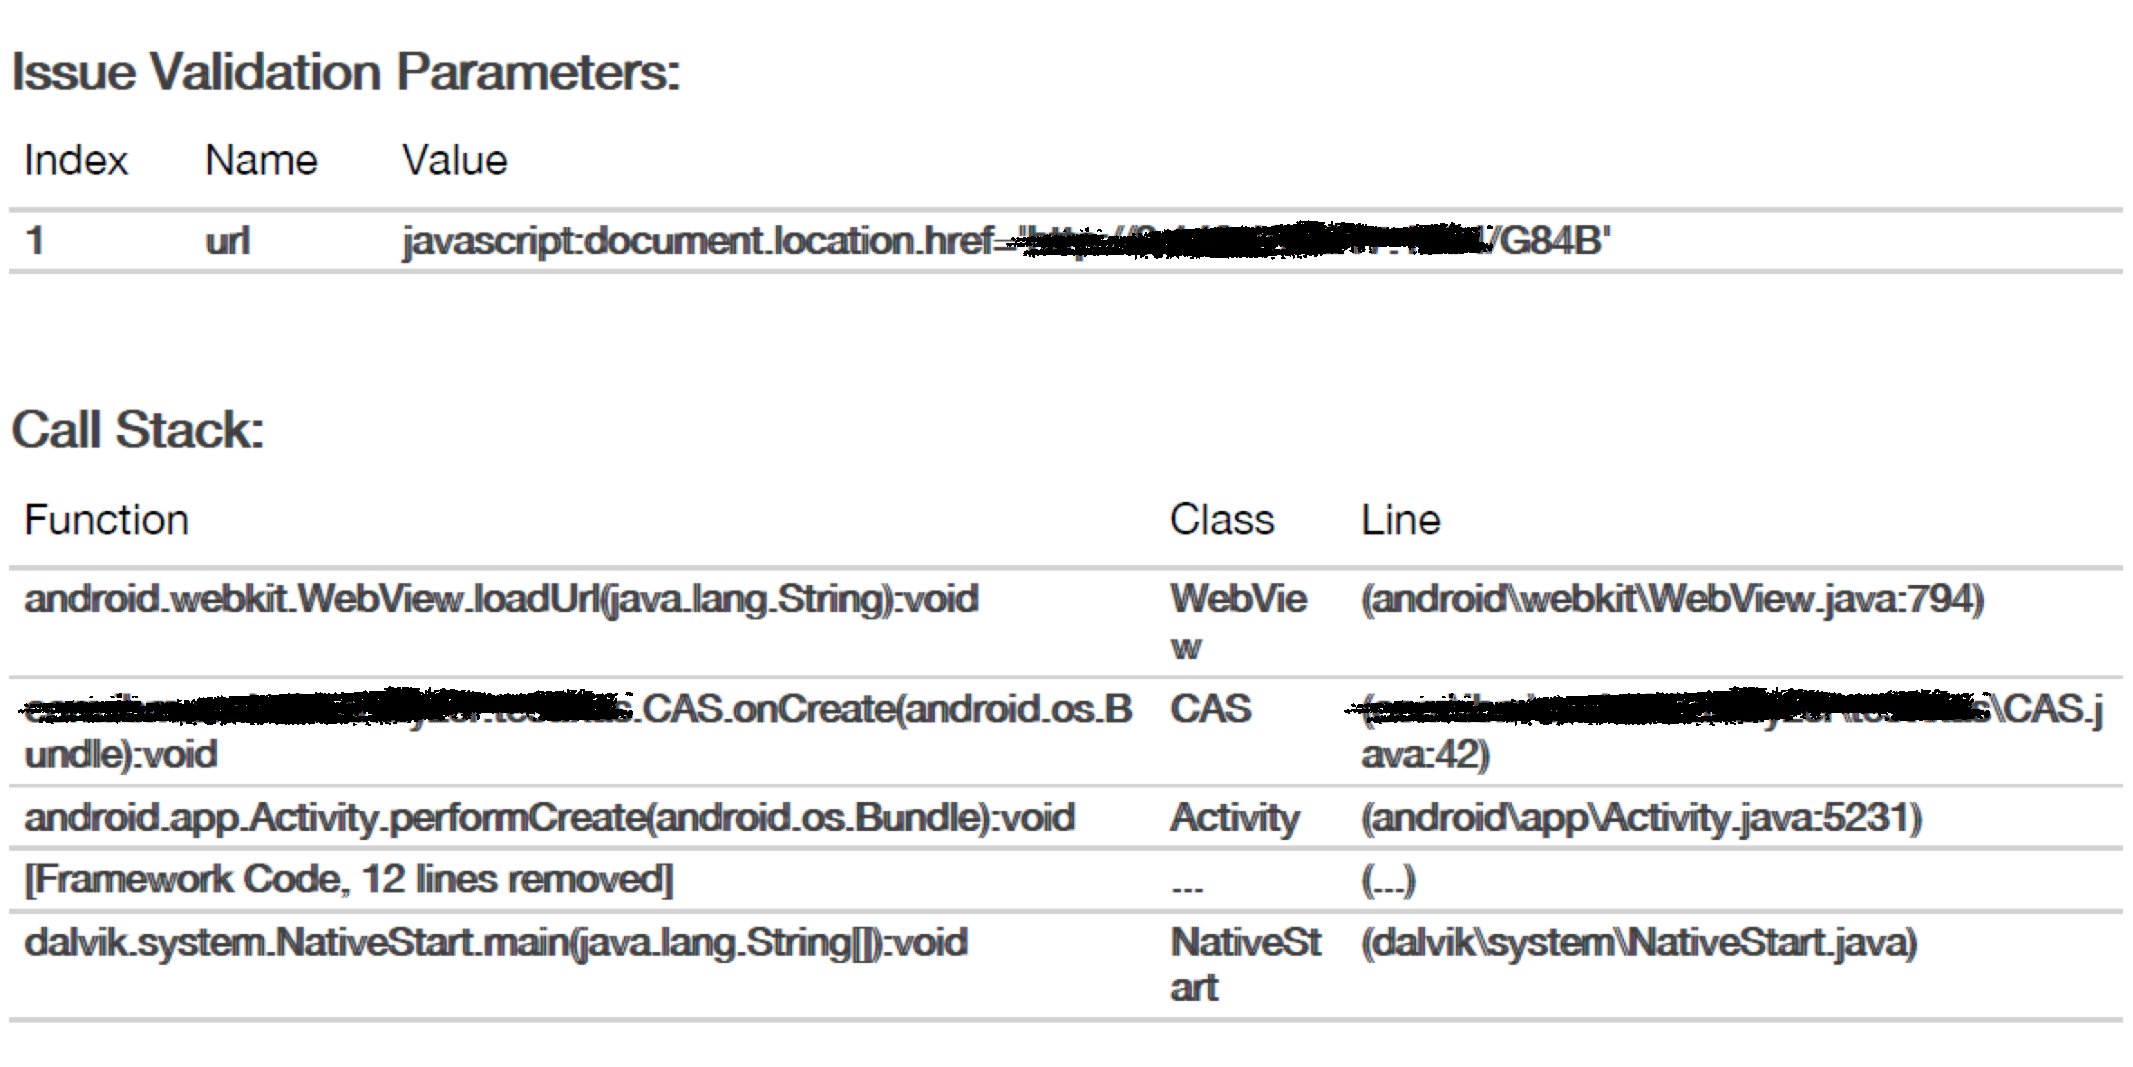
\includegraphics[width=\columnwidth]{screenshot.pdf}
	\caption{\label{Fi:screenshot}A Vulnerability Report Output by \Tool}
\end{figure} 

\subsection{Formal Description}

\algref{maalg} summarizes the complete flow of the \Tool\ algorithm. The starting point is to instrument the target app to record (select) library calls as well as accesses to user-provided data. Next, \Tool\ obtains the declared IAC input points $E$ of the subject application via analysis of its manifest. These seed the iterative testing process. The fixpoint loop iterates over $E$, picking at each iteration a candidate input point $e$ and removing it from the worklist.

\begin{algorithm}[t]
	\DontPrintSemicolon
	\SetKwInOut{Input}{Input}
	\SetKwInOut{Output}{Output}
	\KwIn{$(D,M,V,I)$ \tcp*[h]{testing capabilities}}\;
	\KwIn{$A$ \tcp*[h]{subject mobile app}}\;
	\KwOut{$O$ \tcp*[h]{detected vulnerabilities}}\;
	\Begin{
		$A' \longleftarrow I(A)$ \tcp*[h]{instrument $A$}\; \\
		$E$ $\longleftarrow$ declared interface points of $A$\; \\
		$O \longleftarrow \emptyset$\; \\
		\While{$E \neq \emptyset$}{
			$e$ $\longleftarrow$ choose from $E$\; \\
			$E \longleftarrow E \setminus \{ e \}$\; \\
			\ForEach{$m \in M(e)$}{
				{$b \longleftarrow D(m,e)$}\; \\
				\If{$b$}{
					$p[m,e] \longleftarrow \text{create payload for $e$ with $m$}$\; \\
					$(r,E') \longleftarrow \text{fire $p[m,e]$}$\; \\
					$E \longleftarrow E \cup E'$\; \\
					\If{$V(r)$}{
						$O \longleftarrow O \cup \{ r \}$\;
					}
				}
			}
		}
	}
	\caption{\label{Al:maalg}Outline of the Core \Tool\ Algorithm, where $D$, $M$, $V$ and $I$ Denote Detection, Mutation, Validation and Instrumentation, Respectively}
\end{algorithm}


For the current input point $e$, the next step is to check whether $e$ satisfies the necessary conditions for each attack type $m$. This is represented as the $D(m,e)$ call. Successful detection leads to the creation and application of a payload $p[m,e]$. Exercising the instrumented app $A'$ with $p[m,e]$ yields two artifacts: additional input points $E'$ (discovered by monitoring accesses to custom parameters) and recording of app behaviors/outputs $r$ for validation. The set $O$ of vulnerabilities reported by \Tool\ is augmented if $r$ confirms a vulnerability (the $V(r)$ check).

While \Tool\ is a dynamic testing system with (purposely) limited means to track the internal behavior of the target app, there are still situations in which full coverage is guaranteed. These are governed by a simplifying assumption, stated formally in Definition \ref{De:dataind}, which is too idealized to hold pervasively in reality, but still (i) provides insight into the design of \Tool, and (ii) appears useful in practice given \Tool's recall rate of $>90\%$ over a large set of popular Android apps. (See \secref{evaluation}.)

\begin{definition}[Data Independence]\label{De:dataind} We refer to IAC input point $e$ as \emph{data independent} if execution flow starting at $e$ is decided solely according to (i) boolean extras and/or (ii) presence of extra fields. In particular, the values of non-boolean extras (and other variables in the program) do not affect control flow (cf. \cite{SYGABSV:ISSTA14,W:POPL86}).
\end{definition}

\begin{theorem}[Coverage] Let $e$ be a data-independent input point, such that the value of incoming IAC field $f$, arriving through $e$, flows into sink $s$. 
	Denote by \ETool\ the naive version of \Tool, which enumerates all possible combinations of boolean extras.
	Then \ETool\ is guaranteed to reach $s$ with $f$ mapped to a test payload.\footnote{
		This claim is trivially extensible to \Tool\ by further assuming that boolean extras are related either via independence or via domination.
	}
	\begin{proof}[Proof Sketch] \ETool\ systematically enumerates all boolean combinations. This --- conjoined with the assumption that $e$ is data independent --- guarantees that at some point access to $f$ will be observed. Thus, $f$ will become an attack target (where only the presence, but not the value, of $f$ affects control flow). All continuations of the execution prefix leading to $f$ will be enumerated, which guarantees that a path $p$ starting at $e$, going through a read of $f$ and ending at $s$ will be traversed. Given $f$ is a non-boolean field, \ETool\ will initiate a test execution of $p$ with $f$ mapped to a test payload, which completes the proof.
	\end{proof}
\end{theorem}

%\section{Advanced Features}

Having described the core algorithm, we now highlight challenges that arise in practice and advanced features that we have implemented in response.

\subsection{Indirect Access to Extra Parameters}\label{Se:indirectExtra}

Monitoring accesses to extra parameters is the core means for \Tool\ to expand its coverage of the IAC attack surface. In \secref{corealg}, we illustrate the core functionality of tracking direct access to extra parameters via {\tt Intent} methods like {\tt getStringExtra($\ldots$)}. There is, however, an alternate way of accessing custom parameters, which we demonstrate in \figref{techExample} using the commented-out statements with label {\tt A1}.

Instead of accessing custom parameters via the {\tt Intent} object, the {\tt Bundle} associated with the {\tt Intent} is retrieved via a call to {\tt Intent.getBundle()}. From this point on, custom parameters can be accessed through the {\tt Bundle} object using APIs like {\tt Bundle.getString($\ldots$)}. We refer to this method of accessing custom parameters as \emph{indirect}, because a given {\tt Bundle} may or may not be linked to the {\tt Intent} sent by \Tool.

The first challenge is to establish the binding between the {\tt Intent} sent by \Tool\ and its respective {\tt Bundle}. This is done by installing a monitor inside the {\tt Intent.getBundle()} method. The monitoring code (i) checks whether the receiving {\tt Intent} is indeed the one sent by \Tool\ (by inspecting the {\tt uri} and extra values), and if so, then (ii) the {\tt Bundle} is marked as \emph{relevant}. Furthermore, when a {\tt Bundle} is cloned (which is done via a copy constructor), then the clone is marked as relevant as well. This is achieved by placing monitoring code within the copy constructor.

Based on this marking technique, \Tool\ is able to distinguish between accesses to relevant versus irrelevant {\tt Bundle} objects. Only custom parameters queried over a relevant {\tt Bundle} object are recorded for future investigation. Other custom-parameter accesses are ignored.

\subsection{Coverage Expansion via Boolean Extra Parameters}\label{Se:coverBools}

While string values carried by the {\tt Intent} present an opportunity for an attack, boolean values are not candidate attack targets, and so the naive approach is to simply ignore such input points. In practice, boolean flags are typically used by the code that handles the {\tt Intent} to decide how to process the incoming data. That is, boolean extra parameters often manifest in (or as) path conditions.

As an example, we refer to the commented-out conditional expression in \figref{techExample}, annotated with the {\tt A2} label. It contains four conditional expressions, which refer to boolean extra {\tt ``b1''} in the outer condition and {\tt ``b2''} and {\tt ``b3''} separately and then conjoined in the nested condition. By default all three {\tt execSQL($\ldots$)} sink calls governed by these conditions will be missed by \Tool, as the default value assigned to {\tt ``b1''}, {\tt ``b2''} and {\tt ``b3''} (if they are not set on the {\tt Intent}) is {\tt false}. 

We have verified experimentally, over real-world apps, that coverage loss due to ignoring boolean extras is noticeable. (See \secref{boolExtras}.) On the other hand, 
brute-force enumeration of all possible boolean combinations has exponential complexity, and is therefore undesirable for performance reasons. (Again, see \secref{boolExtras}.) 

\Tool\ aims for a practical tradeoff between performance and coverage. This is achieved in light of two observations:
\begin{itemize}
	\item Domination: We say that boolean extra $b$ \emph{dominates} another boolean extra $b'$ if retrieval of $b'$ from the {\tt Intent} is attempted when $b$ is assigned one of the truth values but not its negation. In the example in \figref{techExample}, {\tt ``b1''} dominates both {\tt ``b2''} and {\tt ``b3''}. The runtime monitoring code installed within the {\tt getBooleanExtra($\ldots$)} method reveals to \Tool\ that access to {\tt ``b2''} and {\tt ``b3''} is made only when {\tt ``b1''} is set to {\tt true}.
	\item Independence: In practice, distinct boolean extras rarely flow into the same path condition. We have validated this experimentally. (See \secref{boolExtras}.) The upshot is that it is more effective to toggle one boolean extra at a time (linear complexity) rather than exhausting all possible value combinations (exponential complexity). As a limitation, \Tool\ would miss cases such as {\tt ``b2''} $\&\&$ {\tt ``b3''} in \figref{techExample}, which require simultaneous toggling of both {\tt ``b2''} and {\tt ``b3''}.
\end{itemize}

The combination of domination and independence leads to the following efficient algorithm for searching through assignments to discovered boolean extras: 
\begin{itemize}
	\item Domination: For an {\tt Intent} that exposes domination of boolean extra $b$ by  $b'$, only $b$ is toggled.
	\item Independence: For an {\tt Intent} that exposes $n$ boolean extras $b_1 \ldots b_n$, where none of the booleans are pairwise related via domination, each of the booleans $b_i$ is negated in turn while retaining the previous value of the other booleans.
\end{itemize}
Independence reduces complexity from exponential to linear, and domination further reduces the number of assignments to be explored, thereby yielding an efficient exploration procedure.

%\section{Advanced Features}

In this section, we describe the design and implementation of the \Tool\ system.

\subsection{The \Tool\ Architecture}

Conceptually, \Tool\ mimics a malicious application. It first collects information about its neighboring apps, as documented by their public IPC interface, and then applies different forms of attack. While testing the app, \Tool\ simultaneously searches for additional attack points beyond the declared ones. This yields an iterative and comprehensive testing process. 

In our initial implementation of \Tool, we packaged its functionality as a mobile app to directly simulate a malicious app installed on the device. For performance and stability reasons, we later rewrote \Tool\ as an external testing algorithm that utilizes the Android Debug Interface (ADB) capabilities, and in particular the Activity Manager ({\tt am}), to gain access to the target app. A 

\Tool\ consists of four main modules: instrumentation, mutation, detection and validation. We survey each in turn below. For now, we suffice with a high-level explanation of how these four modules interlock to enable effective testing. The interaction between the different modules is depicted in \figref{architecture}.

Instrumentation achieves the glass-box effect of monitoring internal app events and behaviors. It is achieved fully automatically, via insertion of debug breakpoints into the app, enabling effective detection of candidate interface points as well as validation of attempted attacks. Attacks are formed via mutation of benign parameters. 

\begin{figure}
\includegraphics[width=\columnwidth]{Architecture.pdf}
\caption{\label{Fi:architecture}High-level architecture of the \Tool\ system}
\end{figure}

The mutation rules are specified in a knowledge database built into the testing engine. These describe how to transform benign IPC messages into attacks as well as how to vary the attack vector to gain more coverage. The knowledge base also specifies how to detect whether an attack vector is potentially relevant, and validate the success of a given attack, which is done with respect to observable events: both those captured by instrumentation hooks and external events, such as writing to the standard log file or sending of HTTP requests.

\subsection{Technical Overview}

We now proceed to an in-depth overview of the main \Tool\ modules. We describe each in turn.

\paragraph{Instrumentation} To insert monitoring code into the target app, \Tool\ utilizes the Java Debug Wire Protocol (JDWP), which is supported by the Dalvik Virtual Machine (VM). Instrumentation hooks are realized as debug breakpoints, which \Tool\ can place into any Android app from the outside without the need to decompile/reassemble it, rewrite its bytecode, or apply any other form of intrusive transformation. 
%
Within a debug breakpoint, \Tool\ has full access to all aspects of the program state, including local variables, the heap graph, the system state, etc. This enables arbitrary detection and validation checks, expressed on a per-rule basis as pure (i.e., side-effect free) Java functionality. 

\TODO{We had many problems deciding when/where to inject a breakpoint. We should talk about that too.}

\paragraph{Detection}

\paragraph{Validation}

\paragraph{Mutation}



\textit{Log Listener}. We listen to the Android log facilitiy (a.k.a
logcat) in order to catch exceptions in native code. Such exceptions
usually indicate memory corruption vulnerabilities.

\textit{HTTP Server.} In order to catch Cross-Application Scripting
(XAS) vulnerabilities in propietary embedded browsers (i.e. ones which
are not implemented on top of \textit{WebView}) we include our on
HTTP Server. We use this server in the following way; Our XAS specific
payload contains a JavaScript (JS) code that redirects the browser
to our HTTP Server. Thus an incoming request on our HTTP Server reflects
an execution of our JS payload, i.e. a vulnerability to XAS.

\textit{Security Rules. }The Security knoweldge is provided to the
The Mobile Analyzer engine by a set of rules. Each rule is composed
of Detection, Mutation, Validation methods. The Detection method indicates
the Scan Manager to whether invoke the Rule's Mutation on a specific
application component and data. The Mutation methods changes the Payload's
data (explained in Section \ref{sub:Modus-Operandi}) to a Rule specified
data. The Validation method validates whether the app component invocation
with the mutated data has caused a security vulnerablitiy. In addition,
each rule includes a set of breakpoints to place when invoking the
target application component with the mutated data.


\subsection{Modus Operandi\label{sub:Modus-Operandi}}

The security testing has multiple interleaved phases.

\textit{Exploration}. In this phase the tool learns the various external
interfaces of the target application.Initially it statically parses
the Android Manifest file (\texttt{AndroidManifest.xml}) and tries
to find public application components (at the time of writing we only
support scanning activities). For each detected component it generates
a Payload object which reflects the component and the target data
that we will mutate during the testing stage. At first the target
data is the Intent's \texttt{data} field. \textit{Testing}. In this
phase the tool goes over all of available Payloads and Rules and runs
the detection method of each rule on the Payload. If the detection
has passed, for each Mutation defined by the Rule, the tool changes
the Payload's data and exercises (in debug mode) the target application
with the mutated Payload. In addition, It places a set of defined
as per defined by the Rule. The total number of generated tests is
therefore 
\[
N=\sum_{\underset{D(r,p)=T}{p\in P,r\in R:}}|M(r)|
\]


where $P$ and $R$ are the payloads and rules sets respectively and
$M(r)$ and $D(r)$ are the mutation and detection of rule $r$. 

For example, in order to test for SQL Injection kind of vulnerabilities,
the malicious input will contain and apostrophe character ('). and
the set of breakpoints will include the \texttt{SQLiteDatabase.execSQL}
API.\textit{ Validation}. In this phase the tools tries to infer whether
the target app is susceptible to security vulnerabilities by using
either the Debugger, Log Listener, or HTTP Server. For instance, if
the target app is susceptible to SQL Injection, using the Debugger,
during the testing, a breakpoint will be hit on some of the SQL sensitive
APIs, such as \texttt{SQLiteDatabase.execSQL.}During the breakpoint
hit, the Debugger exfiltrates the method's arguments, revealing that
the apostrophe was not sanitizied, which proves that the target app
is vulnerable to SQL Injection.

\begin{algorithm}[t]
\DontPrintSemicolon
\SetKwInOut{Input}{Input}
\SetKwInOut{Output}{Output}
\KwIn{$(R,I)$ \tcp*[h]{testing capabilities}}\;
\KwOut{$out$ \tcp*[h]{detected vulnerabilities}}\;
\Begin{
{$E \longleftarrow \textup{declared interface points}$}\; \\
{$out \longleftarrow \emptyset$}\; \\
\While{$E \neq \emptyset$}{
		$e \longleftarrow \textup{choose from}\ E$\; \\
		$E \longleftarrow E \setminus \{ e \}$\; \\
		\ForEach{$(D,M,V) \in $R}{
			\If{$D(e)$}{
				\ForEach{$m \in M(e)$}{
					$p(e,m) \longleftarrow \textup{create payload}$\; \\
					$r \longleftarrow \textit{attack($p(e,m)$, $I$)}$\; \\
					\If{$V($r$,$e$,$E$)$}{
						$out \longleftarrow out \cup \{ r \}$\; \\					
					}
				}
			}
		}
	}
}
\caption{\label{Al:maalg}Outline of the algorithm with extras, where $D$, $M$, $V$ and $E$ are the detection, mutation, validation and instrumentation modules, respectively}
\end{algorithm}


\subsection{Optimizations}

\paragraph{Test Pruning via Probe Templates}

\TODO{Another item here...}

%\subsubsection{Increasing Scan Coverage: Extra Parameters Dynamic Detection}
%
As mentioned in Section {[}ADD XREF HERE{]}, Intent objects include
data in two different fields; in the \textit{data} \texttt{Uri} field
and in the \textit{extras} \texttt{Bundle}. During the \textit{Exploration
}phase our artifact parses the \texttt{AndroidManifest.xml} file in
order to infer the various public interfaces of the target app. The
\texttt{AndroidManifest.xml} only gives our agent intel about the
existence of attackable\textit{ data} \texttt{Uri} fields. Attacking
the \textit{extras} \texttt{Bundle}, a legitimate input to the target
app, however, is by far more challenging, since the tool must realize
about the \texttt{Bundle}'s keys; such keys are not listed on the
Android Manifest file. 

The general approach that our tool takes in order to tackle this challenge
is to dynamically reason about the used \textit{extras} keys, by putting
breakpoints using the \textit{Debugger}, on relevant APIs that consume
data from the \textit{extras }\texttt{Bundle}. Generally whenever
our tool encounters a new extras, it genereates a new Payload that
targets that extra. The scan stops when it reaches the fix-point,
i.e. no more new extras have been dynamically learned.

Whenever the application code reads an extra, e.g. by calling \texttt{Intent.getStringExtra(String
key)}, our tool must link that extra with its Intent instance. While
this is fairly easy for the direct \texttt{Intent.get}\texttt{\textit{{[}Type}}\texttt{{]}Extra}
calls (by observing the 'this' parameter during the breakpoint), it's
more complicated for indirect extra fetches via their embedding Bundle.
The common practice is as follows:

\begin{lstlisting}
Intent i = this.getIntent();
Bundle b = i.getExtras();
String url = b.getString(``url'')
\end{lstlisting}
In order to link the extra with its Intent instance, our tool dynamically
constructs the following tree; the\textit{ }tool first saves the \textit{Remote
Unique ID} {[}ADD EXTERNAL REFERENCE / EXPLANATION HERE{]} of the
\texttt{Bundle} object within the \texttt{Intent}. This is the root
of the tree. Each Bundle clone (done by the Bundle's constructor)
is added as a child. Whenever a \texttt{Bundle.get{[}}\texttt{\textit{Type}}\texttt{{]}(String
key)}is called, we can link back to the Intent by traversing the tree
up to the root {[}ADD NICE GRAPH HERE{]}. This mechanism works fairly
well as per the implementation of the \texttt{Intent.getExtras()}
method:
\begin{lstlisting}
public Bundle getExtras() {
  return (mExtras != null) ? new Bundle(mExtras) : null; }
\end{lstlisting}
Our general Algorithm \ref{AlgorithmExtraParams} supports three configurations;
The configurations differ by their $bruteforce$ procedure. The first
configuration only detects String extras, thus $bruteforce$ is the
empty implementation. The second and third configuration also detect
Boolean extras. The difference between the last two configurations
is the way the algorithm treats extra booleans. In the second configuration,
as depicted by Procedure \ref{AlgorithmBruteforceLinear}, for each
newly detected Boolean extra, we will invoke another test with its
negative value and the current path condition. We call this configuration
\textit{linear bruteforce} as the number of test is linear in the
number of newly booleans. This configuration assumes \textit{independence}
of boolean extras, i.e. it will achieve maximum coverage for the code
depicted by Figure \ref{fig:Indepedent-boolean-extras}. In the third
configuration, as depicted by Procedure \ref{AlgorithmBruteforceExp},
we try all of the possible boolean assignments of the newly detected
Boolean extras. We call this configuration \textit{exponential bruteforce}
as the number of tests is exponential in the number of newly detected
booleans. This configuration assumes \textit{dependence} of new Boolean
extras, i.e. it will acheive maximum coverage for the code depicted
by Figure \ref{fig:Depedent-boolean-extras}

\begin{algorithm}[t]
\DontPrintSemicolon
\SetKwInOut{Input}{Input}
\SetKwInOut{Output}{Output}
\KwIn{$(r,e,E)$}\;
\Begin{
	{$H \longleftarrow \textup{Extra Params Storage}$}\; \\
	{$B \longleftarrow \emptyset$}\; \\
	{$S \longleftarrow \emptyset$}\; \\
	{$X \longleftarrow \textit{Get Extra Parameter Results from r}$}\; \\
	{$P \longleftarrow \textit{Get Extra Parameter Strings Results from e}$}\; \\
	\ForEach{$g \in X$}{
		{$x=(n,t,v) \longleftarrow\textit{Get Type, Name and Value from g}$}\; \\
		\If{$(n,t)\not\in H$} {
			{$H \longleftarrow H\cup{\{n\}}$}\; \\
			{$a \longleftarrow\textit{Get Target App Component from g)}$}\; \\
			\If{$t\textbf{ is }\textit{Boolean}$} {
				{$B \longleftarrow B \cup{\{x\}}$}\; \\
			}
			\If{$t\textbf{ is }\textit{String}$} {
				{$S \longleftarrow S \cup{\{x\}}$}\; \\
			}
		}
	}
	\ForEach{$s \in S$}{
		{$\psi \longleftarrow \textit{Generate a Payload for (e,s)}$}\; \\
		{$E \longleftarrow E \cup{\{\psi\}}$}\;
	}
	\ForEach{$s \in S \cup P$}{
		{$bruteforce(B,H,E,e,s)$}\;
	}

}	
\caption{\label{Al:maalg}Outline of extras detection algorithm implemented as a validation rule V}
\label{AlgorithmExtraParams}
\end{algorithm}

\begin{procedure}[t]
\DontPrintSemicolon
\Begin{
	\ForEach{$b \in B$}{
		{$v \longleftarrow \textup{Get extra param value from b}$}\;
		{$n \longleftarrow \textup{Get extra param name from b}$}\;
		{$\psi \longleftarrow \textit{Generate a Payload from }(e,s,(n,\lnot v))$}\;
		{$E \longleftarrow E \cup{\{\psi\}}$}\;
	}
}	
\caption{bruteforceLinear(B,H,E,e,s)}
\label{AlgorithmBruteforceLinear}
\end{procedure}

\begin{procedure}[t]
\DontPrintSemicolon
\Begin{
	\ForEach{\textup{Boolean assignment} a on B \textup{except the current assignment}} {
		{$\psi \longleftarrow \textit{Generate a Payload from }(e, s, a)$}\;
		{$E \longleftarrow E \cup{\{\psi\}}$}\;
	}
}	
\label{AlgorithmBruteforceExp}
\caption{bruteforceExponential(B,H,E,e,s)}
\end{procedure}

\begin{figure}
\begin{lstlisting}
Boolean foo = intet.getBooleanExtra(``foo'', False)
if (foo) {
  Boolean bar = intet.getBooleaExtra(``bar'', False)
  Boolean baz = intet.getBooleanExtra(``baz'', False)
  if (bar == True) {
    /* security vulnerabiltiy here */ }
if (baz == True) {
  /* another security vulnerabiltiy here */ } }
\end{lstlisting}
\caption{\label{fig:Indepedent-boolean-extras}Indepedent boolean extras (bar
and baz)}
\end{figure}


\begin{figure}
\begin{lstlisting}
Boolean foo = intet.getBooleanExtra(``foo'', False)
if (foo) {
  Boolean bar = intet.getBooleanExtra(``bar'', False)
  Boolean baz = intet.getBooleanExtra(``baz'', False)
  if ((bar == True) && (baz == True)) {
    /* security vulnerabiltiy here */ } }
\end{lstlisting}
\caption{\label{fig:Depedent-boolean-extras}Depedent boolean extras (bar and
baz)}
\end{figure}



%\subsubsection{Test Pruning by Probing}
%
The naive approach is that $D(r,p)$ is always $T$, which results
in $N=|P|\sum_{r\in R}|M(r)|$ tests which can be cumbersome if the
number of mutations is large. Thus creating a sophisticated detection
rule $D(r,p)$ can potentially reduce the number of generated tests. 

The key observation here is that one benign test probe can indiciate
to multiple tests whether or not they have a potential to detect a
true positive. The idea is to compute the API reachability of each
payload. As a first step, each payload is mutated with a benign string
that uniquely identifies the tool, e.g. \texttt{http://GB<ID>/}. Then,
the tool invokes the payload with all breakpoints set. The tool then
saves the list of hit breakpoints for each payload. As a further optimization,
it can save only hit breakpoints that have received the unique string.
The second step is that for each payload, to only invoke rules that
their list of defined breakpoints intersects with the list of saved
payload hit breakpoints. While this approach is not sound, our ampiric
results (Section XX) show only a slight decrease in true positives
with a drastic improvement in performance.


\subsubsection{Test Pruning by Rule Joining}
%


\section{Experimental Evaluation}\label{Se:evaluation}

In this section, we describe quantiative results and share qualitative insight from our evaluation of \Tool. 

\subsection{Experimental Setup and Methodology}

For our experiments, we assembled a suite of 80 Android apps: 4 enterprise apps, 3 apps shipping with version 4.4 of the Android platform, as well as the 73 top-popular Google Play apps in the geography of one of the authors.
The experiments were conducted on a Samsung Nexus 5 device running version 4.4 of the Android platform (CyanogenMod 11). For accuracy and reproducibility, we reset the device to a clean image before testing each of the apps.

Prior to running \Tool, an independent professional ethical hacker audited all 80 apps. The audit resulted in a total of 163 IAC vulnerabilities. \tableref{vulns} provides a breakdown of the results by issue type.

\subsection{Performance Results}

We have conducted a series of experiments to measure, and thereby justify, the key features of \Tool. We organize our description of the experiments around four research hypotheses. The starting point is a baseline algorithm that only targets declared input points via the {\tt data} field.

\paragraph{H1: Probing Boosts Performance} To quantify the performance gain thanks to probing, we enhanced the baseline algorithm with necessary-conditions specifications as described in \secref{detectionSubsec}. Instead of blindly attempting all possible test payloads, the enhanced version first analyzes the probing trace to focus testing only on relevant attack types.

The statistics demonstrate significant improvement. While naive fuzzing expends an average of 64 tests and 24 minutes per app, the enhanced version requires $<15$ tests and $<7$ minutes per app to detect the same set of IAC vulnerabilities.

\paragraph{H2: String Extras are Often Vulnerable} The naive testing algorithm, equipped with probing capabilities, is able to detect a total of 94 out of the 163 known vulnerabilities for a recall rate of $0.57$. Enhancing it to incorporate string extras as attack targets pushes recall up to 0.85, as 46 new vulnerabilities are detected.

The resulting variant features an iterative testing loop, which attacks targets discovered in previous probing/testing rounds. Naturally, this renders it more expensive than its naive counterpart with an average of 26 (compared to 15) tests and 12 (compared to 7) minutes per app.

\paragraph{H3: Boolean Extras Manifest in Path Conditions} The algorithm featuring both probing and manipulation of string extras already detects 140 out of the 163 known vulnerabilities. A natural means to further increase coverage is by exploring new execution paths.

Augmenting the testing algorithm to explore different combinations of boolean extras achieves this goal effectively. This is seen through the discovery of 11 new vulnerabilities, constituting a 7\% improvement in recall, for a total of 151 vulnerabilities detected fully automatically. 

The cost, as expected, is noticeable. The average number of tests per app climbs by x2.42 from 26 to 63 with a proportional rise of x2.1 in testing time from 12 to 25 minutes. This motivates more efficient detection of new paths.

\paragraph{H4: Linear-time Path Exploration is Effective} The fourth and final hypothesis concerns the relationship between boolean extras in their capacity as branching expressions. The claim is that it is effective to treat boolean extras as either dominating each other or being independent.

Under this assumption, which enables toggling of boolean extras one at a time and thus linear-complexity path exploration, testing time drops to 19 minutes (24\% improvement) and the average number of tests is only 40 compared to 63 before (37\% improvement). At the same time, only one of the 151 vulnerabilities detected via the exponential-time path-exploration algorithm is missed for a negligible drop of $<1$\% in recall.

\paragraph{Discussion} In conclusion, \Tool\ effectively balances performance against coverage.\footnote{
	Beyond the data we present here, which confirms our design choices one atop the other, we have a full matrix of measurements per every combination of the choices we've made. We have omitted most of these measurements for lack of space, but note that they are in strong support of our hypotheses.
} Regarding false negatives, our analysis of the 14 misses (w.r.t. the most comprehensive \Tool\ configuration) reveals that these are caused by one or both of the following reasons: (i) incomplete path coverage (and in particular, path conditions other than boolean extras) and (ii) overly conservative probing checks (where the probe is nontrivially mutated by the app, yet it is possible to craft a successful test payload).

A visual illustration of the performance/coverage tradeoffs achieved by the different variants is provided in \figref{trends}, where \Tool\ is labeled ``Linear PC''.
%
``String Extras'' stands out as the variant that maximizes the recall/performance gap. Even though performance increase exceeds gain in coverage when switching to ``Linear PC'', we still view this option as preferable, as less true warnings are missed in return for affordable performance slowdown.

\begin{figure}
	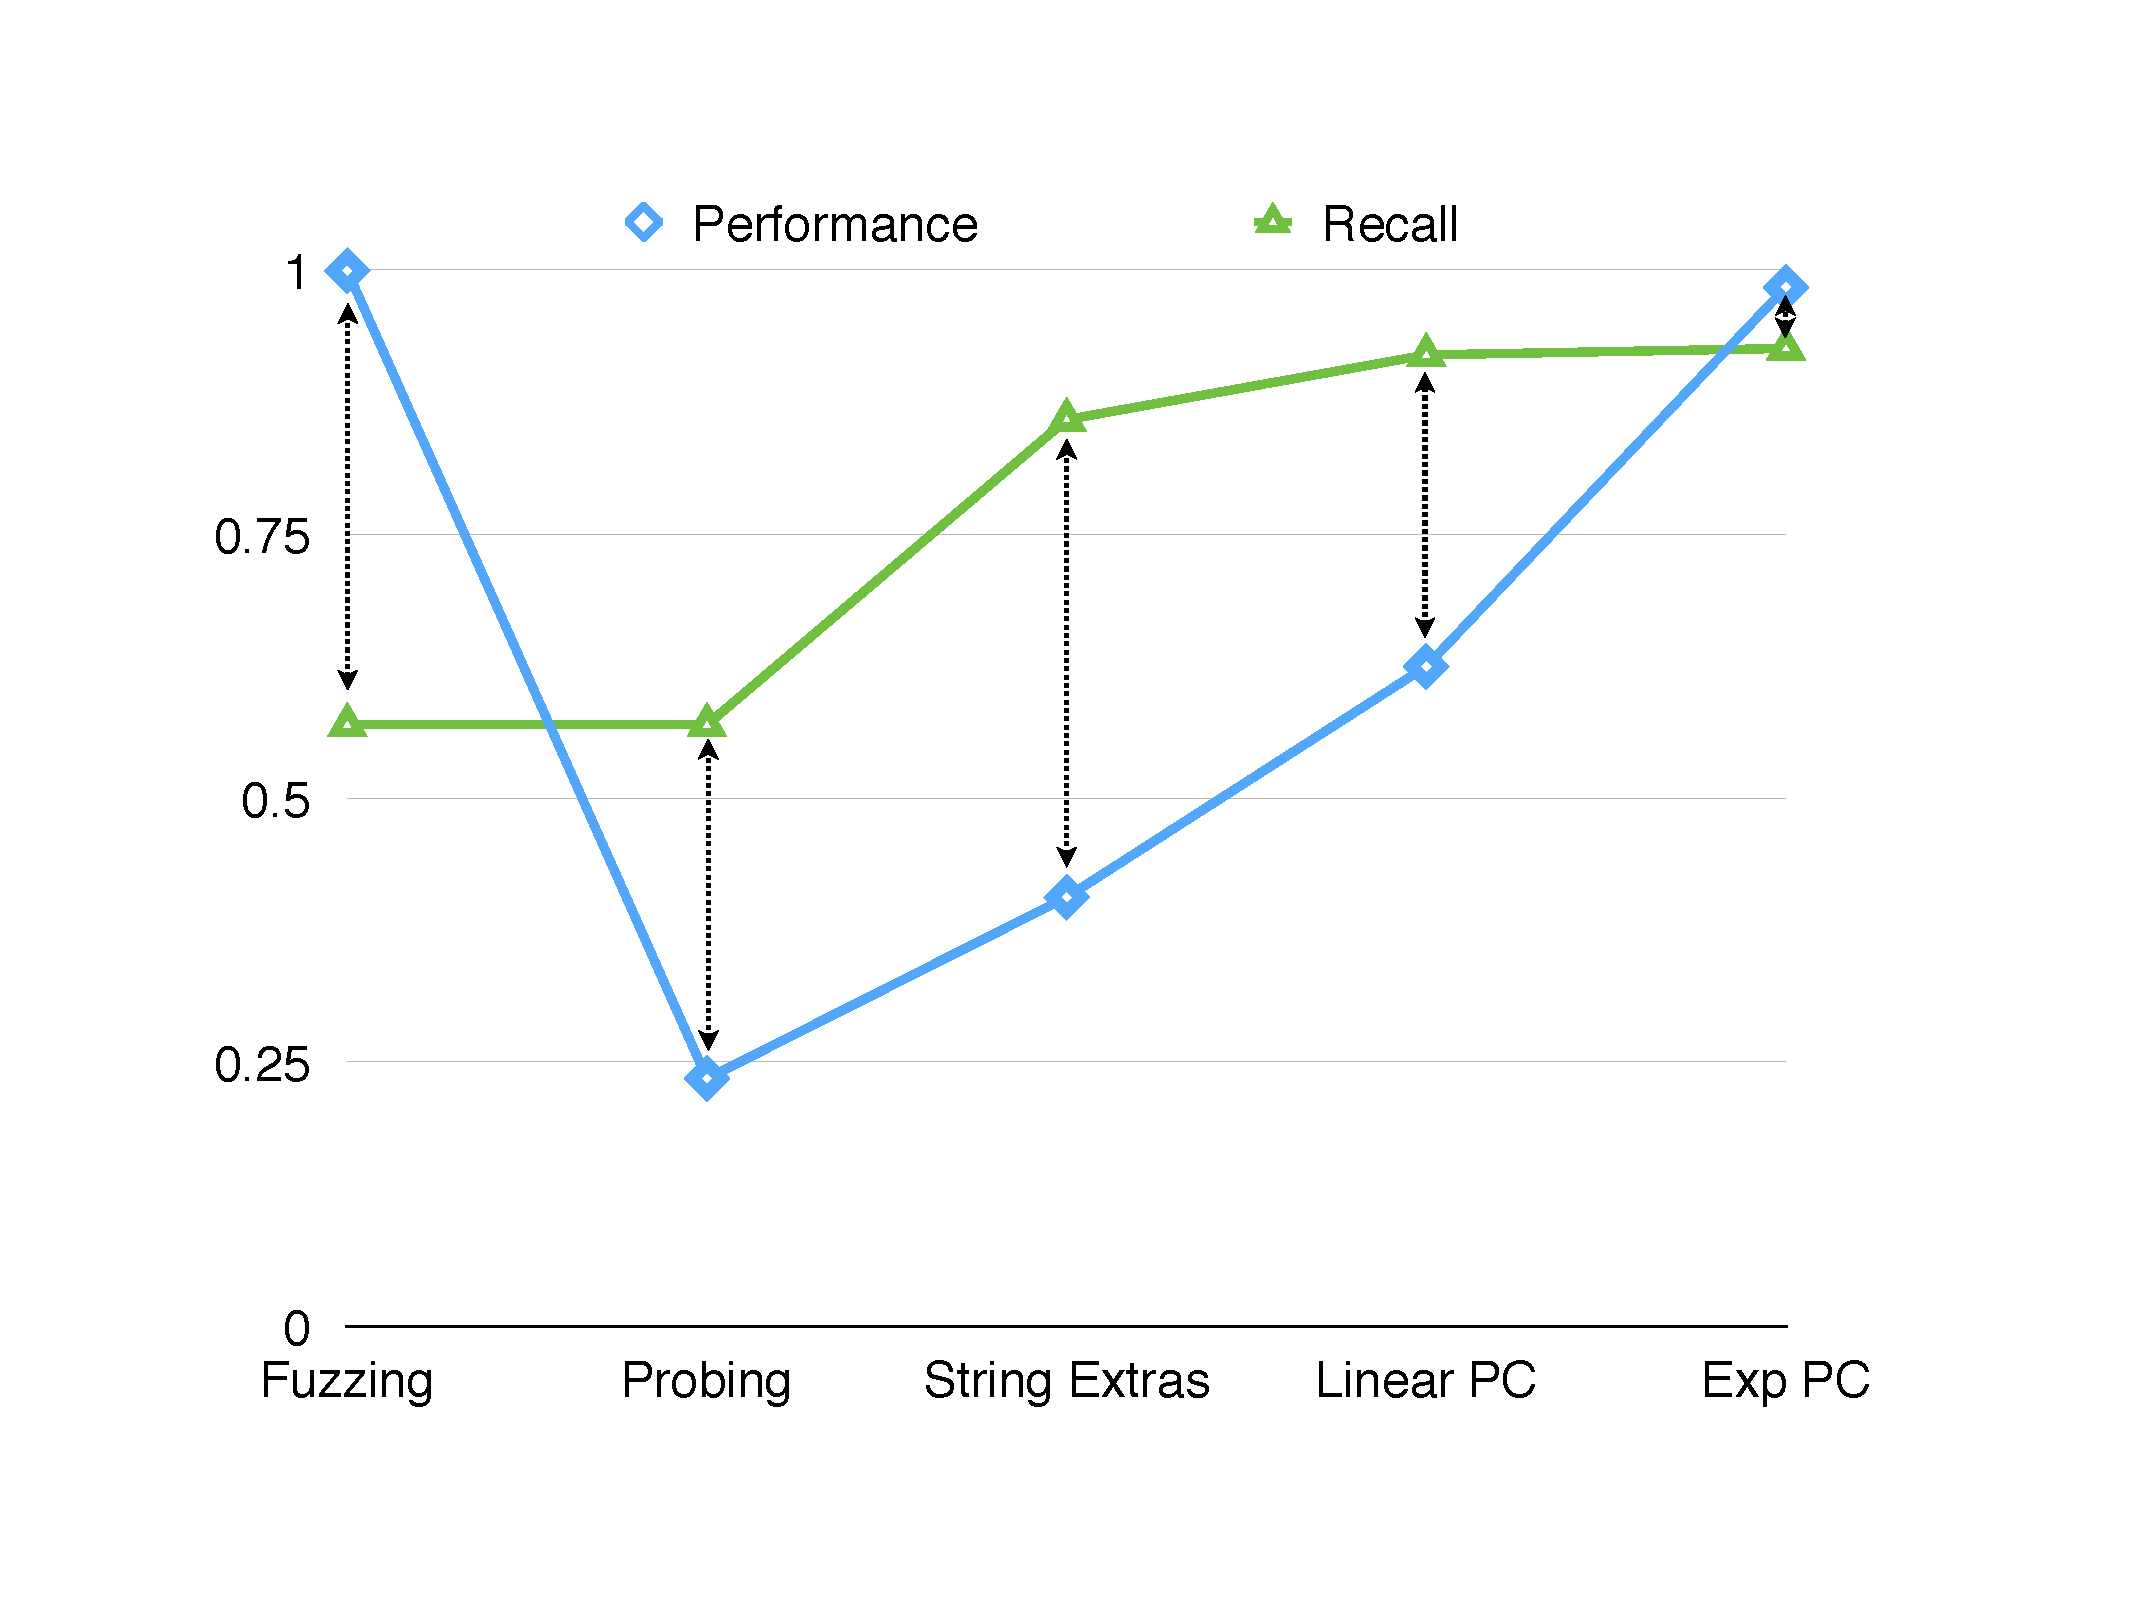
\includegraphics[width=\columnwidth]{trendline.pdf}
	\caption{\label{Fi:trends}Visual Performance/Recall Comparison between Testing Variants}
\end{figure}


\begin{table*}
\begin{scriptsize}
\begin{center}
\begin{tabular}{l|c|c|c|c|c|c|c|c|c|c}
\multicolumn{1}{c|}{\multirow{2}{*}{App Name}} & \multirow{2}{*}{Version} & \multirow{2}{*}{Count} & \multirow{2}{*}{XAS} & \multirow{2}{*}{SQLi} & Unsafe  & UI  & {\tt Fragment}  & Java  & Native  & File  \\
 &  & & &  &  Refl. &  Spoof. &  Injection &  Crash &  Crash &  Man. \\
\hline
com.dropbox.android & 230800 & 4 & \xmark & \xmark & \xmark & \xmark & \cmark & \cmark & \xmark & \xmark \\
com.ebay.mobile & 43 & 3 & \xmark & \xmark & \cmark & \xmark & \xmark & \cmark & \xmark & \xmark \\
com.evernote & 15120 & 7 & \xmark & \xmark & \xmark & \xmark & \cmark & \cmark & \xmark & \xmark \\
com.facebook.katana & 228325 & 4 & \xmark & \xmark & \xmark & \xmark & \xmark & \cmark & \xmark & \xmark \\
com.google.android.gm & 974 & 2 & \xmark & \xmark & \xmark & \xmark & \cmark & \cmark & \xmark & \xmark \\
com.lotus.sync.traveler & 2013062023 & 1 & \xmark & \xmark & \xmark & \xmark & \xmark & \cmark & \xmark & \xmark \\
com.linkedin.android & 56 & 6 & \xmark & \xmark & \xmark & \xmark & \xmark & \cmark & \xmark & \xmark \\
com.nytimes.android & 5523 & 2 & \cmark & \xmark & \xmark & \xmark & \xmark & \cmark & \xmark & \xmark \\
com.google.android.youtube & 4517 & 2 & \xmark & \xmark & \xmark & \xmark & \xmark & \cmark & \xmark & \xmark \\
com.adobe.air & 3700209 & 0 & \xmark & \xmark & \xmark & \xmark & \xmark & \xmark & \xmark & \xmark \\
com.adobe.psmobile & 10 & 0 & \xmark & \xmark & \xmark & \xmark & \xmark & \xmark & \xmark & \xmark \\
com.adobe.reader & 77016 & 3 & \xmark & \xmark & \xmark & \xmark & \xmark & \cmark & \xmark & \xmark \\
com.antivirus & 180265 & 0 & \xmark & \xmark & \xmark & \xmark & \xmark & \xmark & \xmark & \xmark \\
com.android.chrome & 1453090 & 1 & \xmark & \xmark & \xmark & \xmark & \xmark & \cmark & \xmark & \xmark \\
clalit.android & 12 & 0 & \xmark & \xmark & \xmark & \xmark & \xmark & \xmark & \xmark & \xmark \\
com.alibaba.aliexpresshd & 56 & 1 & \xmark & \xmark & \xmark & \xmark & \xmark & \cmark & \xmark & \xmark \\
com.android.vending & 80280020 & 3 & \xmark & \xmark & \xmark & \xmark & \cmark & \cmark & \xmark & \xmark \\
com.box.android & 30200 & 1 & \xmark & \xmark & \xmark & \xmark & \xmark & \cmark & \xmark & \xmark \\
com.cleanmaster.security & 10400566 & 0 & \xmark & \xmark & \xmark & \xmark & \xmark & \xmark & \xmark & \xmark \\
com.fibi & 8 & 0 & \xmark & \xmark & \xmark & \xmark & \xmark & \xmark & \xmark & \xmark \\
com.fitbit.FitbitMobile & 1772 & 1 & \xmark & \xmark & \xmark & \xmark & \xmark & \cmark & \xmark & \xmark \\
com.fitnesskeeper.runkeeper.pro & 215 & 0 & \xmark & \xmark & \xmark & \xmark & \xmark & \xmark & \xmark & \xmark \\
com.google.android.apps.docs.editors.sheets & 1314426 & 4 & \xmark & \xmark & \xmark & \xmark & \xmark & \cmark & \xmark & \xmark \\
com.google.android.apps.m4b & 62 & 0 & \xmark & \xmark & \xmark & \xmark & \xmark & \xmark & \xmark & \xmark \\
com.google.android.apps.magazines & 2014051213 & 0 & \xmark & \xmark & \xmark & \xmark & \xmark & \xmark & \xmark & \xmark \\
com.google.android.apps.maps & 800001324 & 2 & \xmark & \xmark & \xmark & \xmark & \xmark & \cmark & \xmark & \xmark \\
com.google.android.apps.plus & 413004558 & 10 & \xmark & \xmark & \xmark & \xmark & \cmark & \cmark & \cmark & \xmark \\
com.google.android.GoogleCamera & 22024130 & 0 & \xmark & \xmark & \xmark & \xmark & \xmark & \xmark & \xmark & \xmark \\
com.google.android.maps.mytracks & 74 & 3 & \xmark & \xmark & \xmark & \cmark & \xmark & \cmark & \xmark & \xmark \\
com.google.android.music & 1514 & 4 & \xmark & \xmark & \xmark & \xmark & \xmark & \cmark & \xmark & \xmark \\
com.google.android.talk & 21224130 & 1 & \xmark & \cmark & \xmark & \xmark & \xmark & \xmark & \xmark & \xmark \\
com.google.earth & 13294050 & 1 & \xmark & \xmark & \xmark & \xmark & \xmark & \cmark & \xmark & \xmark \\
com.hipmunk.android & 102 & 0 & \xmark & \xmark & \xmark & \xmark & \xmark & \xmark & \xmark & \xmark \\
com.ideomobile.hapoalim & 117 & 12 & \cmark & \xmark & \xmark & \cmark & \xmark & \cmark & \xmark & \xmark \\
com.ideomobile.leumicard & 42 & 2 & \cmark & \xmark & \xmark & \xmark & \xmark & \cmark & \xmark & \xmark \\
com.intsig.camscanner & 3302 & 1 & \xmark & \xmark & \xmark & \xmark & \xmark & \cmark & \xmark & \xmark \\
com.leumi.leumiwallet & 18 & 1 & \xmark & \xmark & \xmark & \xmark & \xmark & \cmark & \xmark & \xmark \\
com.melodis.midomiMusicIdentifier.freemium & 10602 & 2 & \cmark & \xmark & \xmark & \xmark & \xmark & \cmark & \xmark & \xmark \\
com.mxtech.videoplayer.ad & 700000070 & 2 & \xmark & \xmark & \xmark & \xmark & \cmark & \cmark & \xmark & \xmark \\
com.netgate & 141 & 0 & \xmark & \xmark & \xmark & \xmark & \xmark & \xmark & \xmark & \xmark \\
com.nike.plusgps & 99 & 0 & \xmark & \xmark & \xmark & \xmark & \xmark & \xmark & \xmark & \xmark \\
com.onoapps.cal4u & 5 & 0 & \xmark & \xmark & \xmark & \xmark & \xmark & \xmark & \xmark & \xmark \\
com.paypal.android.p2pmobile & 49 & 1 & \xmark & \xmark & \xmark & \xmark & \xmark & \cmark & \xmark & \xmark \\
com.runtastic.android & 90 & 1 & \xmark & \xmark & \xmark & \xmark & \xmark & \cmark & \xmark & \xmark \\
com.snapchat.android & 323 & 0 & \xmark & \xmark & \xmark & \xmark & \xmark & \xmark & \xmark & \xmark \\
com.ubercab & 30618 & 0 & \xmark & \xmark & \xmark & \xmark & \xmark & \xmark & \xmark & \xmark \\
com.urbandroid.sleep & 842 & 4 & \xmark & \xmark & \xmark & \xmark & \cmark & \cmark & \xmark & \xmark \\
com.viber.voip & 61 & 2 & \xmark & \xmark & \xmark & \xmark & \xmark & \cmark & \xmark & \xmark \\
com.waze & 1019718 & 1 & \xmark & \xmark & \xmark & \xmark & \xmark & \cmark & \xmark & \xmark \\
com.yahoo.mobile.client.android.flickr & 41700 & 0 & \xmark & \xmark & \xmark & \xmark & \xmark & \xmark & \xmark & \xmark \\
com.yelp.android & 10000903 & 4 & \xmark & \xmark & \xmark & \xmark & \xmark & \cmark & \xmark & \xmark \\
com.android.contacts & 19 & 7 & \xmark & \xmark & \xmark & \cmark & \xmark & \cmark & \xmark & \xmark \\
com.android.dialer & 19 & 2 & \xmark & \xmark & \xmark & \xmark & \xmark & \cmark & \xmark & \xmark \\
com.facebook.orca & 221196 & 1 & \xmark & \xmark & \cmark & \xmark & \xmark & \xmark & \xmark & \xmark \\
com.facebook.pages.app & 232657 & 1 & \xmark & \xmark & \cmark & \xmark & \xmark & \xmark & \xmark & \xmark \\
org.mozilla.firefox & 2013061803 & 6 & \xmark & \xmark & \xmark & \cmark & \xmark & \cmark & \xmark & \cmark \\
com.gau.go.launcherex & 234 & 2 & \xmark & \xmark & \xmark & \xmark & \xmark & \cmark & \xmark & \xmark \\
com.google.android.apps.currents & 130781200 & 0 & \xmark & \xmark & \xmark & \xmark & \xmark & \xmark & \xmark & \xmark \\
com.google.android.apps.docs & 1218226 & 5 & \xmark & \xmark & \xmark & \cmark & \xmark & \cmark & \xmark & \xmark \\
com.google.android.apps.finance & 35 & 2 & \xmark & \xmark & \xmark & \xmark & \xmark & \cmark & \xmark & \xmark \\
com.google.android.apps.translate & 20700177 & 2 & \xmark & \xmark & \cmark & \xmark & \xmark & \cmark & \xmark & \xmark \\
org.dayup.gtask & 1602 & 11 & \xmark & \xmark & \xmark & \xmark & \cmark & \cmark & \xmark & \xmark \\
com.ibm.lotus.connections.mobile & 2013092105 & 5 & \xmark & \xmark & \xmark & \xmark & \xmark & \cmark & \xmark & \xmark \\
com.ibm.android.sametime.meetings & 20130528 & 3 & \xmark & \xmark & \xmark & \xmark & \xmark & \cmark & \xmark & \xmark \\
com.ibm.android.sametime & 2013041715 & 1 & \xmark & \xmark & \xmark & \xmark & \xmark & \cmark & \xmark & \xmark \\
com.ibm.mobile.android.unyte & 20121206 & 0 & \xmark & \xmark & \xmark & \xmark & \xmark & \xmark & \xmark & \xmark \\
com.imdb.mobile & 103220310 & 0 & \xmark & \xmark & \xmark & \xmark & \xmark & \xmark & \xmark & \xmark \\
com.instagram.android & 197069 & 3 & \xmark & \xmark & \xmark & \xmark & \xmark & \cmark & \xmark & \xmark \\
com.android.mms & 19 & 3 & \xmark & \xmark & \xmark & \cmark & \xmark & \cmark & \xmark & \xmark \\
mobi.mgeek.TunnyBrowser & 331 & 1 & \xmark & \xmark & \xmark & \xmark & \xmark & \cmark & \xmark & \xmark \\
com.opera.browser.beta & 1600559192 & 0 & \xmark & \xmark & \xmark & \xmark & \xmark & \xmark & \xmark & \xmark \\
org.telegram.messenger & 227 & 0 & \xmark & \xmark & \xmark & \xmark & \xmark & \xmark & \xmark & \xmark \\
org.zwanoo.android.speedtest & 124 & 1 & \xmark & \xmark & \xmark & \xmark & \xmark & \cmark & \xmark & \xmark \\
com.shazam.android & 78059 & 5 & \cmark & \xmark & \xmark & \xmark & \xmark & \cmark & \xmark & \xmark \\
com.skype.raider & 50469393 & 0 & \xmark & \xmark & \xmark & \xmark & \xmark & \xmark & \xmark & \xmark \\
com.sgiggle.production & 53 & 3 & \xmark & \xmark & \xmark & \xmark & \xmark & \cmark & \xmark & \xmark \\
com.ted.android & 18 & 0 & \xmark & \xmark & \xmark & \xmark & \xmark & \xmark & \xmark & \xmark \\
com.devuni.flashlight & 139 & 0 & \xmark & \xmark & \xmark & \xmark & \xmark & \xmark & \xmark & \xmark \\
com.whatsapp & 47672 & 0 & \xmark & \xmark & \xmark & \xmark & \xmark & \xmark & \xmark & \xmark \\
fr.beungoud.xbmcremote & 47 & 0 & \xmark & \xmark & \xmark & \xmark & \xmark & \xmark & \xmark & \xmark \\ 
\hline\hline
\multicolumn{1}{c|}{{\bf 55/80}} & {\bf 163} & {\bf 5} & {\bf 1} & {\bf 4}  & {\bf 6}  & {\bf 8} & {\bf 30} & {\bf 1} & {\bf 1} \\
%\_Dropbox v2.3.8 & 4 & \xmark & \xmark & \xmark & \xmark & \cmark & \cmark & \xmark & \xmark \\
%\_eBay v2.3.0.25 & 3 & \xmark & \xmark & \cmark & \xmark & \xmark & \cmark & \xmark & \xmark \\
%\_Evernote v5.1.2 & 7 & \xmark & \xmark & \xmark & \xmark & \cmark & \cmark & \xmark & \xmark \\
%\_Facebook v3.3 & 4 & \xmark & \xmark & \xmark & \xmark & \xmark & \cmark & \xmark & \xmark \\
%\_Gmail v4.5-836823 & 2 & \xmark & \xmark & \xmark & \xmark & \cmark & \cmark & \xmark & \xmark \\
%\_IBM Notes Traveler v9.0.0.0 201306202317 & 1 & \xmark & \xmark & \xmark & \xmark & \xmark & \cmark & \xmark & \xmark \\
%\_LinkedIn v3.0.2 & 6 & \xmark & \xmark & \xmark & \xmark & \xmark & \cmark & \xmark & \xmark \\
%\_NYTimes for Android v3.2.2 & 2 & \cmark & \xmark & \xmark & \xmark & \xmark & \cmark & \xmark & \xmark \\
%\_YouTube v4.5.17 & 2 & \xmark & \xmark & \xmark & \xmark & \xmark & \cmark & \xmark & \xmark \\
%Adobe AIR v3.7.0.209 & 0 & \xmark & \xmark & \xmark & \xmark & \xmark & \xmark & \xmark & \xmark \\
%Adobe Photoshop Express v1.3.3 & 0 & \xmark & \xmark & \xmark & \xmark & \xmark & \xmark & \xmark & \xmark \\
%Adobe Reader v10.6.0 & 3 & \xmark & \xmark & \xmark & \xmark & \xmark & \cmark & \xmark & \xmark \\
%Antivirus Security - FREE v3.2.3 & 0 & \xmark & \xmark & \xmark & \xmark & \xmark & \xmark & \xmark & \xmark \\
%Chrome Browser - Google v27.0.1453.90 & 1 & \xmark & \xmark & \xmark & \xmark & \xmark & \cmark & \xmark & \xmark \\
%clalit.android-1. & 0 & \xmark & \xmark & \xmark & \xmark & \xmark & \xmark & \xmark & \xmark \\
%com.alibaba.aliexpresshd-1. & 1 & \xmark & \xmark & \xmark & \xmark & \xmark & \cmark & \xmark & \xmark \\
%com.android.vending-1 & 3 & \xmark & \xmark & \xmark & \xmark & \cmark & \cmark & \xmark & \xmark \\
%com.box.android-1. & 1 & \xmark & \xmark & \xmark & \xmark & \xmark & \cmark & \xmark & \xmark \\
%com.cleanmaster.security-1. & 0 & \xmark & \xmark & \xmark & \xmark & \xmark & \xmark & \xmark & \xmark \\
%com.fibi-1 & 0 & \xmark & \xmark & \xmark & \xmark & \xmark & \xmark & \xmark & \xmark \\
%com.fitbit.FitbitMobile-1. & 1 & \xmark & \xmark & \xmark & \xmark & \xmark & \cmark & \xmark & \xmark \\
%com.fitnesskeeper.runkeeper.pro-1. & 0 & \xmark & \xmark & \xmark & \xmark & \xmark & \xmark & \xmark & \xmark \\
%com.google.android.apps.docs.editors.sheets-1. & 4 & \xmark & \xmark & \xmark & \xmark & \xmark & \cmark & \xmark & \xmark \\
%com.google.android.apps.m4b-1. & 0 & \xmark & \xmark & \xmark & \xmark & \xmark & \xmark & \xmark & \xmark \\
%com.google.android.apps.magazines-1. & 0 & \xmark & \xmark & \xmark & \xmark & \xmark & \xmark & \xmark & \xmark \\
%com.google.android.apps.maps-1. & 2 & \xmark & \xmark & \xmark & \xmark & \xmark & \cmark & \xmark & \xmark \\
%com.google.android.apps.plus-1. & 10 & \xmark & \xmark & \xmark & \xmark & \cmark & \cmark & \cmark & \xmark \\
%com.google.android.GoogleCamera-1 & 0 & \xmark & \xmark & \xmark & \xmark & \xmark & \xmark & \xmark & \xmark \\
%com.google.android.maps.mytracks-1. & 3 & \xmark & \xmark & \xmark & \cmark & \xmark & \cmark & \xmark & \xmark \\
%com.google.android.music-1. & 4 & \xmark & \xmark & \xmark & \xmark & \xmark & \cmark & \xmark & \xmark \\
%com.google.android.talk-2. & 1 & \xmark & \cmark & \xmark & \xmark & \xmark & \xmark & \xmark & \xmark \\
%com.google.earth-1. & 1 & \xmark & \xmark & \xmark & \xmark & \xmark & \cmark & \xmark & \xmark \\
%com.hipmunk.android-1. & 0 & \xmark & \xmark & \xmark & \xmark & \xmark & \xmark & \xmark & \xmark \\
%com.ideomobile.hapoalim-1. & 12 & \cmark & \xmark & \xmark & \cmark & \xmark & \cmark & \xmark & \xmark \\
%com.ideomobile.leumicard-1 & 2 & \cmark & \xmark & \xmark & \xmark & \xmark & \cmark & \xmark & \xmark \\
%com.intsig.camscanner-1. & 1 & \xmark & \xmark & \xmark & \xmark & \xmark & \cmark & \xmark & \xmark \\
%com.leumi.leumiwallet-1. & 1 & \xmark & \xmark & \xmark & \xmark & \xmark & \cmark & \xmark & \xmark \\
%com.melodis.midomiMusicIdentifier.freemium-1. & 2 & \cmark & \xmark & \xmark & \xmark & \xmark & \cmark & \xmark & \xmark \\
%com.mxtech.videoplayer.ad-1. & 2 & \xmark & \xmark & \xmark & \xmark & \cmark & \cmark & \xmark & \xmark \\
%com.netgate-1 & 0 & \xmark & \xmark & \xmark & \xmark & \xmark & \xmark & \xmark & \xmark \\
%com.nike.plusgps-1. & 0 & \xmark & \xmark & \xmark & \xmark & \xmark & \xmark & \xmark & \xmark \\
%com.onoapps.cal4u-1 & 0 & \xmark & \xmark & \xmark & \xmark & \xmark & \xmark & \xmark & \xmark \\
%com.paypal.android.p2pmobile-1 & 1 & \xmark & \xmark & \xmark & \xmark & \xmark & \cmark & \xmark & \xmark \\
%com.runtastic.android-1. & 1 & \xmark & \xmark & \xmark & \xmark & \xmark & \cmark & \xmark & \xmark \\
%com.snapchat.android-1. & 0 & \xmark & \xmark & \xmark & \xmark & \xmark & \xmark & \xmark & \xmark \\
%com.ubercab-1. & 0 & \xmark & \xmark & \xmark & \xmark & \xmark & \xmark & \xmark & \xmark \\
%com.urbandroid.sleep-1. & 4 & \xmark & \xmark & \xmark & \xmark & \cmark & \cmark & \xmark & \xmark \\
%com.viber.voip-1. & 2 & \xmark & \xmark & \xmark & \xmark & \xmark & \cmark & \xmark & \xmark \\
%com.waze-1. & 1 & \xmark & \xmark & \xmark & \xmark & \xmark & \cmark & \xmark & \xmark \\
%com.yahoo.mobile.client.android.flickr-1. & 0 & \xmark & \xmark & \xmark & \xmark & \xmark & \xmark & \xmark & \xmark \\
%com.yelp.android-1. & 4 & \xmark & \xmark & \xmark & \xmark & \xmark & \cmark & \xmark & \xmark \\
%Contacts. & 7 & \xmark & \xmark & \xmark & \cmark & \xmark & \cmark & \xmark & \xmark \\
%Dialer. & 2 & \xmark & \xmark & \xmark & \xmark & \xmark & \cmark & \xmark & \xmark \\
%Facebook Messenger v2.5.3-release & 1 & \xmark & \xmark & \cmark & \xmark & \xmark & \xmark & \xmark & \xmark \\
%Facebook Pages Manager v1.4.1 & 1 & \xmark & \xmark & \cmark & \xmark & \xmark & \xmark & \xmark & \xmark \\
%Firefox Browser for Android v22.0 & 6 & \xmark & \xmark & \xmark & \cmark & \xmark & \cmark & \xmark & \cmark \\
%GO Launcher EX v3.9.11 & 2 & \xmark & \xmark & \xmark & \xmark & \xmark & \cmark & \xmark & \xmark \\
%Google Currents v2.1.0 & 0 & \xmark & \xmark & \xmark & \xmark & \xmark & \xmark & \xmark & \xmark \\
%Google Drive v1.2.182.26 & 5 & \xmark & \xmark & \xmark & \cmark & \xmark & \cmark & \xmark & \xmark \\
%Google Finance v2.2.7 & 2 & \xmark & \xmark & \xmark & \xmark & \xmark & \cmark & \xmark & \xmark \\
%Google Translate v2.7 & 2 & \xmark & \xmark & \cmark & \xmark & \xmark & \cmark & \xmark & \xmark \\
%GTasks v1.6.0.2 & 11 & \xmark & \xmark & \xmark & \xmark & \cmark & \cmark & \xmark & \xmark \\
%IBM Connections v4.4.0 & 5 & \xmark & \xmark & \xmark & \xmark & \xmark & \cmark & \xmark & \xmark \\
%IBM Sametime Meetings v8.5.2.4 & 3 & \xmark & \xmark & \xmark & \xmark & \xmark & \cmark & \xmark & \xmark \\
%IBM Sametime v8.5.2.4 201304171550 & 1 & \xmark & \xmark & \xmark & \xmark & \xmark & \cmark & \xmark & \xmark \\
%IBM SmartCloud Meetings v8.5.2.1.201212060646 & 0 & \xmark & \xmark & \xmark & \xmark & \xmark & \xmark & \xmark & \xmark \\
%IMDB Movies And TV v3.2.2.103220310 & 0 & \xmark & \xmark & \xmark & \xmark & \xmark & \xmark & \xmark & \xmark \\
%Instagram v3.5.3 & 3 & \xmark & \xmark & \xmark & \xmark & \xmark & \cmark & \xmark & \xmark \\
%Mms & 3 & \xmark & \xmark & \xmark & \cmark & \xmark & \cmark & \xmark & \xmark \\
%mobi.mgeek.TunnyBrowser-1. & 1 & \xmark & \xmark & \xmark & \xmark & \xmark & \cmark & \xmark & \xmark \\
%Opera browser beta v15.0.1162.59192 & 0 & \xmark & \xmark & \xmark & \xmark & \xmark & \xmark & \xmark & \xmark \\
%org.telegram.messenger-1. & 0 & \xmark & \xmark & \xmark & \xmark & \xmark & \xmark & \xmark & \xmark \\
%org.zwanoo.android.speedtest-1 & 1 & \xmark & \xmark & \xmark & \xmark & \xmark & \cmark & \xmark & \xmark \\
%Shazam v3.14.0-JB78059 & 5 & \cmark & \xmark & \xmark & \xmark & \xmark & \cmark & \xmark & \xmark \\
%Skype - free IM and video calls v3.2.0.6673 & 0 & \xmark & \xmark & \xmark & \xmark & \xmark & \xmark & \xmark & \xmark \\
%Tango Text Voice and Video v2.10.48610 & 3 & \xmark & \xmark & \xmark & \xmark & \xmark & \cmark & \xmark & \xmark \\
%TED v1.1.6 & 0 & \xmark & \xmark & \xmark & \xmark & \xmark & \xmark & \xmark & \xmark \\
%Tiny Flashlight + LED v4.9.4 & 0 & \xmark & \xmark & \xmark & \xmark & \xmark & \xmark & \xmark & \xmark \\
%WhatsApp Messenger v2.10.222 & 0 & \xmark & \xmark & \xmark & \xmark & \xmark & \xmark & \xmark & \xmark \\
%XBMC remote control v2.0.1 & 0 & \xmark & \xmark & \xmark & \xmark & \xmark & \xmark & \xmark & \xmark \\ 
%\hline\hline
%\multicolumn{1}{c|}{{\bf 55/80}} & {\bf 163} & {\bf 5} & {\bf 1} & {\bf 4}  & {\bf 6}  & {\bf 8} & {\bf 30} & {\bf 1} & {\bf 1} \\
\end{tabular}
\end{center}
\end{scriptsize}
\caption{\label{Ta:vulns}Detected Vulnerabilities with Breakdown by Attack Type}
\end{table*}

\subsection{Interesting Vulnerabilities}\label{Se:caseStudies}

We conclude by highlighting three vulnerabilities of special interest being both nontrivial and severe. We have reported these vulnerabilities to the developers. In all cases, the vulnerable scenario was confirmed to be critical and was fixed shortly thereafter.

\paragraph{Preference Activities and Dynamic Fragment Loading}\label{Se:PreferenceActivities}

The Android framework provides an abstract {\tt Activity} class,\texttt{
android.preference.PreferenceActivity}, which serves as a reusable and extensible preferences dialog. 
The {\tt PreferenceActivity} class queries its input {\tt Intent} for several extra data fields, including \texttt{EXTRA\_SHOW\_FRAGMENT}
(\texttt{show\_fragment}) 
and \texttt{EXTRA\_SHOW\_FRAGMENT\_ARGUMENTS}.
(\texttt{show\_fragment\_arguments}).

The first of these fields specifies the name 
of a \texttt{Fragment} class, which \texttt{PreferenceActivity}
displays dynamically upon being created. The {\tt Fragment.Instantiate($\ldots$)} method creates a {\tt Fragment} instance dynamically, via reflection, and then
casts it into the {\tt Fragment} type.

The second field is the \texttt{Fragment}'s input {\tt Bundle}. A loaded \texttt{Fragment} can
receive input arguments by accessing its host activity (and therefore
its input \texttt{Intent}) using the \texttt{Fragment.getActivity()} API. The second field therefore provides the additional arguments required to instantiate the {\tt Fragment} (if any).

Any app containing an exported {\tt Activity} that extends the {\tt PreferenceActivity} class can be subverted to load an arbitrary class
by exploiting the unsafe dynamic {\tt Fragment} loading process. \Tool\ was indeed able to take advantage of this weakness
in several applications --- including Gmail, Google Translate and Dropbox --- by
targeting the \texttt{show\_fragment}  field with {\tt Fragment} class names from the Android framework and providing corresponding arguments via the \texttt{show\_fragment\_arguments} field. 

%These were loaded successfully, since
%the class loader assigned to the context of \texttt{PreferenceActivity} is the core
%\texttt{PathClassLoader}, which can load any class from the app itself as well as the Android and Java libraries.

As a notable example, \Tool\ was able to inject integrity payloads via the input {\tt Bundle} in Android's built-in Settings app, where {\tt PreferenceActivity} is used. 
The vulnerability detected by \Tool\ allows a malicious app to load an instance of \texttt{ChooseLockPasswordFragment}
and feed data into it despite its normal instantiation under a non-exported
activity. A user can then bypass insertion of the old PIN number when changing PINs by setting the \texttt{confirm\_credentials} field to \texttt{false}.

%\begin{figure}
%	\includegraphics[width=\columnwidth]{CaseStudy1.pdf}
%	\caption{\label{Fi:caseStudy1}Visual Representation of the Testing Scenario Exposing the {\tt Fragment}-injection Vulnerability in the Settings System App}
%\end{figure}

We have reported this severe issue to the Android security team. In response, they
created a patch for \texttt{PreferenceActivity} starting Android 4.4 KitKat. 
The patched class contains a new method, \texttt{isValidFragment(String fragmentName)}, 
which is documented as follows in the Android SDK:
\begin{quote}
	``\textit{Added in API level 19}
	
	Subclasses should override this method and verify that the given fragment
	is a valid type to be attached to this activity. The default implementation
	returns true for apps built for \texttt{targetSdkVersion}
	older than \texttt{KITKAT}. For later versions, it will throw an exception.
	
	\textit{Parameters} \texttt{fragmentName} the class name of the Fragment
	about to be attached to this activity. 
	
	\textit{Returns} true if the fragment class name is valid for this
	Activity and false otherwise which is called before the fragment is
	instantiated.'' 
\end{quote}
It is the responsibility of the developer to override method {\tt isValidFragment($\ldots$)} to whitelist the {\tt Fragment}s that are allowed to be loaded within a specific
{\tt Activity}.

\paragraph{XAS Weakness in Apache Cordova}\label{Se:CordovaXAS}

Apache Cordova is among the most prevalent Android frameworks, serving as the basis of 5.8\% of all Android applications and 1.2\% of the top 500 apps in the Google-Play store.\footnote{\url{http://www.appbrain.com/stats/libraries/details/phonegap/phonegap-apache-cordova}} Cordova exposes a set of APIs that allow the developer to access native device functionality, such as the camera or accelerometer, from JavaScript. Combined with a UI framework like jQuery, Cordova enables the development of smartphone apps based only
on HTML, CSS and JavaScript. This is forming into a strong trend. Indeed as of July 2014, 7.8\% of all new apps (30 days old or younger) are built atop Cordova, which indicates that Cordova is increasingly gaining popularity.

Applications written on top of Cordova make use of a {\tt WebView} instance to interact with the user. When the application is first loaded, it invokes the {\tt loadUrl($\ldots$)} method of the {\tt CordovaWebView} class, which is a subtype of {\tt Activity}. {\tt loadUrl($\ldots$)} has the following implementation:
\begin{small}
\begin{lstlisting}[showstringspaces=false]
public void loadUrl(String url) {
  if (url.equals("about:blank") || 
      url.startsWith("javascript:")) { this.loadUrlNow(url); }
  else {
    String initUrl = this.getProperty("url", null); }
    // If first page of app, 
    // then set URL to load to be the one passed in
    if (initUrl == null) { this.loadUrlIntoView(url); }
    // Otherwise use the URL specified in the extras bundle
    else { this.loadUrlIntoView(initUrl); } }
\end{lstlisting}
\end{small}
As the code shows, the {\tt initUrl} string is defined as the result of a  {\tt getProperty("url", null)} call, which consists of the following code:
\begin{small}
\begin{lstlisting}[showstringspaces=false]
public String getProperty(String name, String defaultValue) {
  Bundle bdl = 
      this.cordova.getActivity().getIntent().getExtras();
  if (bdl == null) { return defaultValue; }
  Object p = bdl.get(name);
  if (p == null) { return defaultValue; }
  return p.toString(); }
\end{lstlisting}
\end{small}
The return value of {\tt getProperty($\ldots$)} is an extra parameter obtained from the {\tt Bundle} object associated with the current {\tt Intent} (which, in turn, is retrieved via the {\tt getIntent().getExtras()} getter chain). Thus, variable {\tt url} in {\tt loadUrl($\ldots$)}, flowing into the {\tt loadUrlIntoView} call, presents an opportunity for an attack. This variable is defined
as the value of the {\tt 'url'} extra parameters, which can be set externally.  
Thus, a malicious caller could launch the {\tt Activity} with an {\tt Intent} whose respective {\tt Bundle} maps {\tt 'url'} to an unintended value. The provided URL will consequently be loaded by Cordova and rendered within the {\tt WebView}.

This vulnerability enables theft of sensitive data (such as login credentials) owned by any Cordova-based app having the vulnerable {\tt WebView} embedded in a public {\tt Activity}.
We emphasize that in the described scenario, the {\tt 'url'} extra parameter is fetched directly from the extras {\tt Bundle}. 

\Tool\ was able to successfully detect this nontrivial vulnerability using its ability to track indirect accesses to extra parameters, as described in \secref{customparams}.
We  disclosed this acute issue to the Cordova team as CVE-2014-3500. The Cordova team has issued a patch starting version 3.5.1 of the framework.

\paragraph{File Manipulation in the Firefox Browser}\label{Se:FirefoxFileManipulation}

Public class {\tt org.mozilla.gecko.CrashReporter} extends {\tt Activity}. Its purpose is to send crash dumps to Mozilla when the Firefox browser treminates unexpectedly.
{\tt CrashReporter}, a subclass of {\tt Activity}, receives the dump file path as input via an extra {\tt Intent} parameter called {\tt minidumpPath}. When this {\tt Activity} is launched, its {\tt onCreate($\ldots$)} method is executed, triggering the following sequence of actions:
\begin{enumerate}
	\item Using the \texttt{moveFile($\ldots$)} method, the current dump file is moved to the pending dump-files path: \texttt{files/mozilla/Crash Reports/pending}.
	\item A metadata filename is derived from the given dump file path by replacing all occurrences of the {\tt .dmp} file extension with  {\tt .extra}. 
	\item The metadata file is subsequently moved to the pending dump-files path using the \texttt{moveFile($\ldots$)} method.
	\item The metadata file is parsed into key/value format. The target server's URL (i.e., the URL of the server that the crash information is sent to) is specified there using the \texttt{ServerURL} key.
	\item The {\tt CrashReporter} dialog is displayed to the user.
	\item Finally, when the user presses either the ``Close'' or the ``Restart'' button with the ``Send report'' checkbox enabled, the dump file --- along with other sensitive information --- are sent to the specified server by invoking the {\tt sendReport($\ldots$)} method. Note that if the user further checks the ``Include the address'' checkbox, then Android logs are sent as well.
\end{enumerate}

The security problem created by this scenario traces back to {\tt CrashReporter} and its treatment of the {\tt minidumpPath} extra parameter as trusted, where in fact it should be treated as untrusted, as it is specified by an external agent.
%
Indeed, an adversarial agent can manipulate the source path of the moved file as well as the deduced extra file. 
This manipulation enables control over the server that the crash dump is reported to, in addition to controlling the path of the crash dump file, which allows theft of sensitive information.

We have disclosed this issue as CVE-2014-1506 to the Mozilla security team, which released a fixed version shortly afterwards.\footnote{\url{https://www.mozilla.org/security/announce/2014/mfsa2014-24.html}} 
	\Tool\ was able to detect this issue by discovering the {\tt minidumpPath} extra parameter and recording calls to {\tt File.renameTo($\ldots$)} and {\tt File.createNewFile()}, wherein the initialized {\tt File} object is mapped to  a user-controlled path.

%\begin{table*}
\begin{center}
\begin{tabular}{|c|c|c|c|c|c|c|c|c|c|c|}
\hline 
Run & Duration (mins) & Attacks & Probes & Hit Probes & Extras & Boolean Extras & TPs & High & Medium & Low\tabularnewline
\hline 
\hline 
No Pruning with no extras &  &  & 0 & 0 & 0 & 0 &  &  &  & \tabularnewline
\hline 
Pruning with no extras & 314 & 708 & 416 & 199 & 0 & 0 & 59 & 4 & 1 & 54\tabularnewline
\hline 
No Pruning with naive extras{*} & 1452 & 3874 & 0 & 0 & 149 & 0 & 87 & 19 & 7 & 61\tabularnewline
\hline 
Pruning with naive extras{*} & 475 & 1065 & 530 & 393 & 130 (-19) & 0 & 75 & 18 (-1) & 6 (-1) & 51 (-10,+3)\tabularnewline
\hline 
No Pruning with linear bruteforce &  &  & 0 & 0 &  &  &  &  &  & \tabularnewline
\hline 
Pruning with linear bruteforce{*}{*} & 1583 & 3257 & 1252 & 1154 & 335 & 137 & 92 & 15 & 9 & 68\tabularnewline
\hline 
No Pruning with exponential bruteforce &  &  & 0 & 0 &  &  &  &  &  & \tabularnewline
\hline 
Pruning with exponential bruteforce{*}{*} & 1914 & 3821 & 1479 & 1377 & 320 & 135 & 92 & 15 & 10 & 67\tabularnewline
\hline 
\end{tabular}
\caption{foo}
\end{center}
\end{table*}

{*} Need to re-run as per change of extras algorithm.

{*}{*} Need to re-run several apps due to Bundle.get bug


\section{Related Work}\label{Se:related}

We survey related studies on Android testing and security. Though we  focus mainly on testing, we also highlight related research in the areas of verification and prevention.

\cheapar{Testing} Maji et al. \cite{MAB:DSN12} conduct an experimental evaluation of the robustness of IAC in Android. In their experiments, they perform fuzz testing with illegal {\tt Intent} inputs, e.g. with blank or random action or data fields, random extras, etc. Their results indicate that exceptional situations are often handled poorly, and under certain conditions can even cause the Android runtime to crash.

Somewhat similarly, Sasnauskas and Regeher \cite{SR:WODA14} develop a fuzzing framework for {\tt Intent}s with the goal of triggering interesting bugs (including crashes) that have previously been unknown. Their fuzzing technique combines static analysis with random test-case generation. Findings due to their system include crashes in dozens of core Google as well as Google Play apps, which in some cases result in complete OS reboot.

Yang et al. \cite{YZWZD:ACCS14} present IntentFuzzer, a fuzzing tool that analyzes mobile applications for \emph{capability leaks} (aka \emph{permission redelegation}). These occur if an app owns the permission to access a sensitive resource (or set of resources) and can be manipulated into performing such an access on behalf of another application that lacks the permission. Yang et al. report that 161 out of 2,000 Google Play apps they tested have this weakness.

Ye et al. \cite{YCZJ:MOMM13} create a fuzzer specifically for {\tt Activity}s that accept external MIME data. These are discovered via analysis of the {\tt <intent-filter>} tag in the manifest file. Experiments conducted by the authors, where they generated abnormal audio and video data as input, reveal 14 bugs. These include application crashes and freezes, as well as excessive consumption of system resources.

The AppsPlayground framework, developed by Rastogi et al. \cite{RCE:CODAPSY13}, performs dynamic security analysis of Android apps to detect malware as well as grayware apps.  AppsPlayground has a modular deign, enabling usage of different exploration techniques, including event triggering, fuzz testing and context-sensitive crawling. The choice of detection technique is also modular, permitting e.g. taint tracking, API monitoring and kernel-level monitoring. 

\cheapar{Verification} The ComDroid tool, developed by Chin et al. \cite{CFGW:MOBISYS11}, detects IAC vulnerabilities statically. Specifically, ComDroid performs bounded interprocedural flow-sensitive tracking of {\tt Intent} objects with sensitivity to {\tt Intent} properties, such as whether the {\tt Intent} contains extra parameters or defines an action. The Epicc analysis tool, by Octeau et al. \cite{Epicc}, has a similar scope. It achieves better scalability than ComDroid by modeling the discovery of communication instances as Interprocedural Distributive Environment (IDE) problems \cite{IDE}.
%A warning is issued if an implicit {\tt Intent} is sent out with no or weak permission requirements.

The CHEX system, developed by Lu et al. \cite{LLWLJ:CCS12}, vets Android apps for component hijacking vulnerabilities by means of flow- and context-sensitive data-flow analysis. The authors report on an evaluation of CHEX over 5,486 Android apps, 254 of which were found vulnerable.  

\cheapar{Prevention} % http://dl.acm.org/citation.cfm?id=2381948
Kantola et al. \cite{KCHW:SPSM12} address IAC vulnerabilities due to (i) exposure of app-internal messages to third parties or (ii) receipt of external messages by internal components of the app. As a solution, they propose to harden the Android heuristics to determine the eligible senders and recipients of messages.

Another proposal, by Cozzette et al. \cite{CLMOABFKNR:IM13}, is to revise {\tt Intent} handling such that the system can only err on the safe side. Contrary to the current design, whereby a developer may inadvertently create opportunities for another app to inject a malicious {\tt Intent} or intercept outgoing {\tt Intent}s, Cozzette et al. propose a model that disables all such behaviors unless these are requested explicitly by the developer. This does not remove integrity threats, however, as erroneous handling of incoming {\tt Intent}s remains possible.

Luo et al. study the {\tt WebView} component, which enables an app to embed a browser in its UI (cf. Section \ref{Se:surface}). They observe that {\tt WebView} diverges from standard browsers in that both sandbox protection and the client-side Trusted Component Base (TCB) are weakened, and identify security threats that arise as a consequence. They also propose potential solutions to prevent such attacks.

\section{Conclusion and Future Work}\label{Se:conclusion}

We have presented \Tool, a comprehensive testing algorithm for (inbound) IAC integrity threats, which is available as a commercial cloud service. \Tool\
maintains a feedback loop, such that custom IAC parameters detected on the fly are later explored and tested. Path exploration is governed by efficient manipulation of boolean IAC parameters. \Tool\ currently tests for eight different IAC attack vectors. In our experiments over 80 top-popular apps, we have established the justification for different design choices that \Tool\ embodies, and have demonstrated \Tool\ to be effective overall with the ability to detect 150/163 known IAC vulnerabilities in the benchmark suite (recall rate of $>92\%$).

In the future, we plan to extend \Tool\ to handle more aspects of Android IAC, including (i) fuzzing of integral extra parameter; (ii) attacking other components beyond {\tt Activity}s; and (iii) accounting for multi-app attack scenarios, such that the payload flows across multiple appllications (not only components, which \Tool\ supports already; cf. \cite{RALB:ARES14}). In addition, we intend to search for analogous forms of attack in other platforms (mainly iOS).




%\newpage

\balance

\bibliographystyle{abbrv}
\bibliography{bibliography}

\end{document}
